\section{Методы обнаружения сигналов}
\label{sec:theory}

\newcommand{\AR}{\mathit{AR}}
\newcommand{\MA}{\mathit{MA}}
\newcommand{\ARMA}{\mathit{ARMA}}
\newcommand{\FT}{\mathcal{F}}


\subsection{Общие сведения}

Обнаружение сигналов является фундаментальной задачей радиосвязи. Потребность в этом возникает в большинстве сценариев использования радиосредств, причем, каждая сфера применения определяет эту проблему по-своему. Пользовательским радиоприемникам нужно сканировать заданный диапазон на наличие наиболее мощных сигналов, которые достаточно сильно выделяются на общем фоне и непрерывны во времени. В служебной связи задача осложняется тем, что зачастую канал можно обнаружить только во время его использования. При дальней связи и связи в неблагоприятных условиях полоса частот известна заранее, но мощность сигнала меньше мощности шума, тогда обнаружить его означает подобрать подходящую модель, чтобы компенсировать помехи и извлечь полезную информацию. В сфере радиоразведки ведется постоянная гонка вооружений и данная проблема актуальна всегда.

Такое многообразие задач, имеющих общее название "<обнаружение сигналов">, очевидно, не может быть охвачено небольшим набором методов. Тем не менее, в их решении есть общая основа  --- представление сигнала. Радиоволна имеет вполне определенные физические характеристики, которые исследователь может представить в любой удобной для него форме.
Наиболее интуитивное их выражение --- это последовательность мгновенных уровней сигнала во времени. Оно полезно тем, что существует много методов для работы с временными рядами. Таким образом можно использовать достижения других областей науки и привносить в них свои новшества. Такой подход называется представлением сигнала во временном домене.
В этой форме, однако, не очевидно, как энергия волн распределена по частотам. А это свойство очень полезно, так как нас интересует, на каких частотах наблюдается активность. Поэтому, широкое применение нашел альтернативный подход --- представление сигнала в частотном домене. Оно не привносит новой информации, а является альтернативной формой записи параметров радиоволн. Переход от одного представления к другому осуществляется через прямое и обратное преобразование Фурье, о котором более подробно будет рассказано ниже.

Эти представления лежат в основе двух семейств методов: анализа временных рядов и спектрального анализа. Они решают разные задачи и дополняют друг друга.


\subsection{Авторегрессионная модель}

Авторегрессионная модель (Autoregressive model, $\AR$) --- это математическая модель случайного процесса, основывающаяся на предположении, что последующее значение последовательности линейно зависит от предыдущих (\autoref{eq:theory:ar}). \cite{weber_time_series}

\begin{equation}
  \label{eq:theory:ar}
  X_t = \sum_{i=1}^p \phi_i X_{t-i} + \varepsilon_t
\end{equation}
\begin{explanation}
\item[где] $\phi_1, \dotsc, \phi_p$ --- параметры модели;
\item $\varepsilon_t$ --- шум.
\end{explanation}

Это достаточно простая конструкция, которая, впрочем, демонстрирует неплохие результаты и применяется как составная часть более сложных моделей.
Ее основные достоинства --- невысокая вычислительная сложность и возможность применения к любому временному ряду без его анализа. Так можно получать базовое качество оценки параметров ряда и использовать его для получения предварительных выводов.
Недостатки вытекают из простоты --- неспособность уловить сложные закономерности и неустойчивость к шуму.


Настройка авторегрессии заключается в подборе ее параметров. Это делается с помощью метода наименьших квадратов. Количество параметров называется порядком модели и записывается $\mathit{\AR}(n)$. Порядок подбирается вручную или методами выбора модели (AIC, BIC и другими). Он не должен быть слишком большим --- в этом случае невязка с данными, используемыми для настройки будет мала, а на новых сильно возрастет. Эта проблема известна как переобучение, то есть излишняя подстройка под обучающие данные, в результате чего страдает обобщающая способность модели.

Теоретически $\AR$ обоснована только для случайных процессов, обладающих свойством слабой стационарности, то есть математическое ожидание не изменяется во времени и функция автоковариации постоянна для сдвига $k$:

\begin{equation}
  \begin{split}
    E[X_t] & = const \\
    cov(X_{t_1}, X_{t_1-k}) & = cov(X_{t_2}, X_{t_2-k})
  \end{split}
\end{equation}

Это утверждение неверно применительно к радиосигналам, поэтому авторегрессионная модель в реальных ситуациях обладает слабой предсказательной силой, но по ее поведению все-равно можно сделать некоторые выводы о природе случайного процесса. Например, наблюдая за значениями невязки модельных и реальных данных можно заметить разладки в СП --- невязка резко возрастет.

Тем не менее, на очищенных от шума данных авторегрессия работает неплохо. $\AR(2)$ достаточно хорошо приближает модельный FM сигнал (\autoref{fig:theory:ar_pred_next}). Визуально отличия заметны только при детальном рассмотрении. Это можно объяснить гладкой формой синусоиды: каждое следующее значение не сильно отклоняется от предыдущих. При добавлении шума результат становится значительно хуже.

\begin{figure}[h]
  \centering
  \begin{subfigure}{0.45\textwidth}
    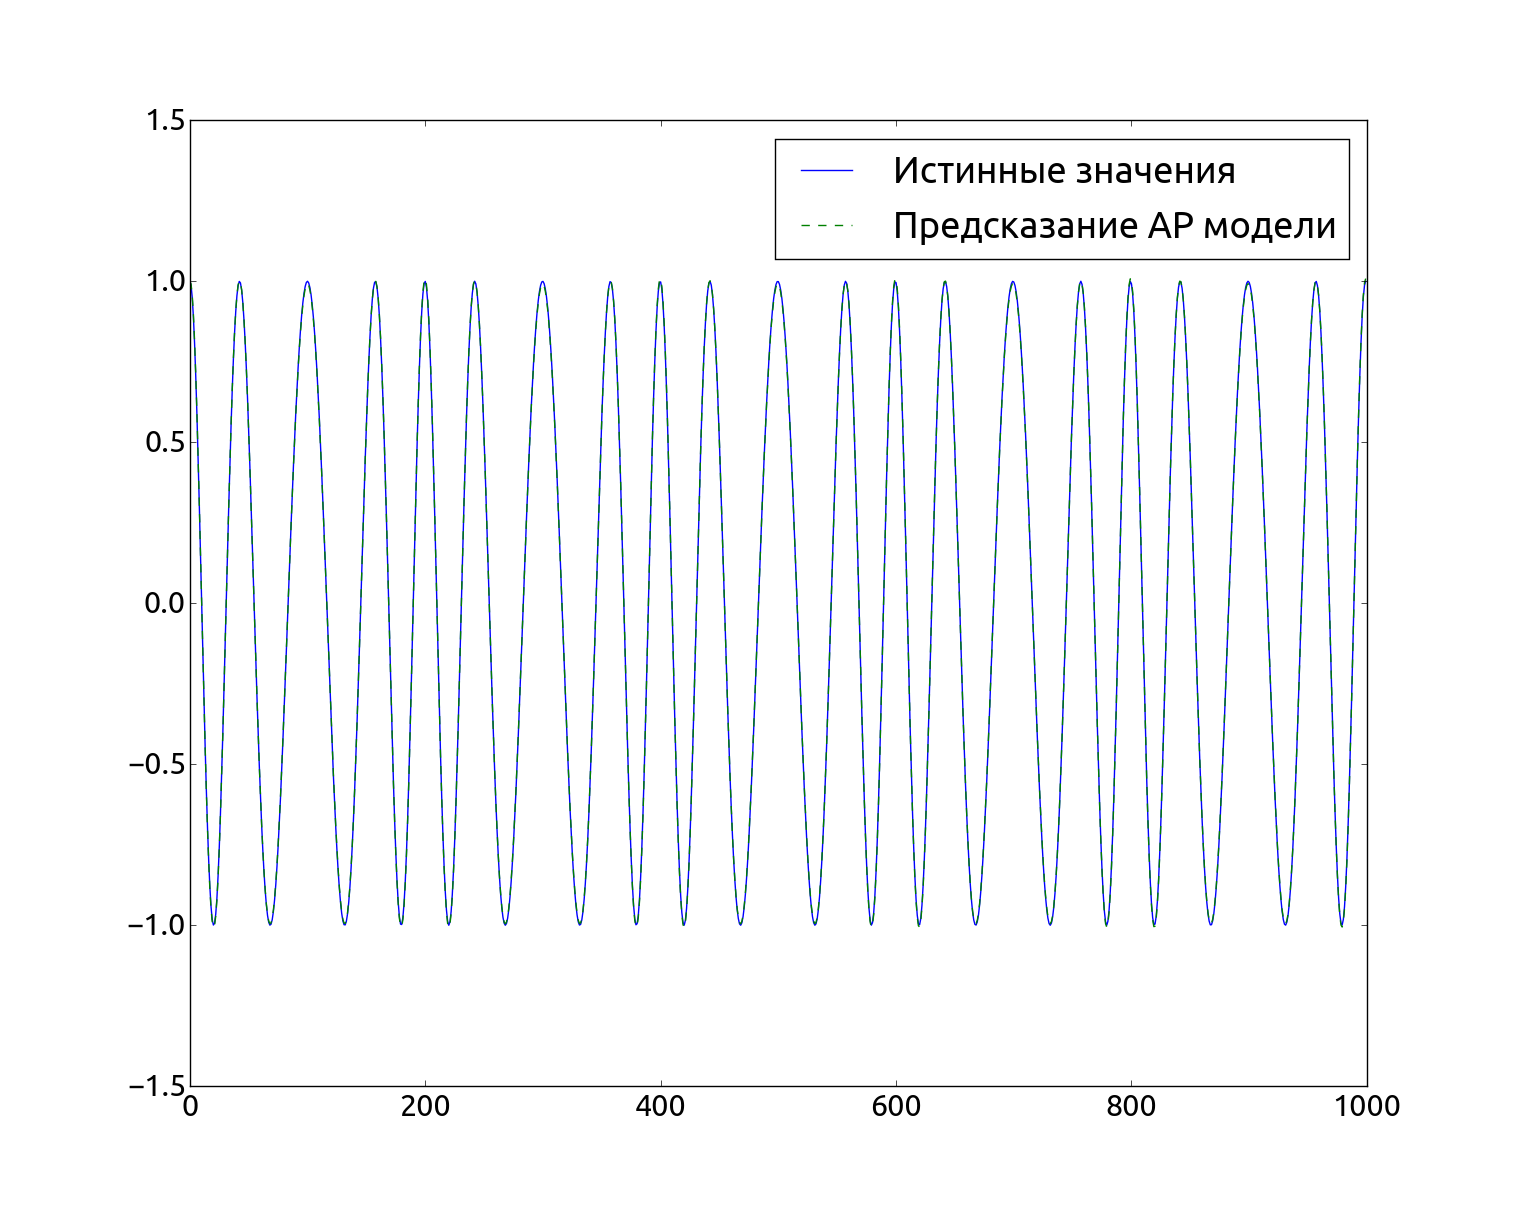
\includegraphics[width=\textwidth]{theory/ar_pred_next}
    \caption{}
    \label{fig:theory:ar_pred_next_whole}
  \end{subfigure}
  \begin{subfigure}{0.45\textwidth}
    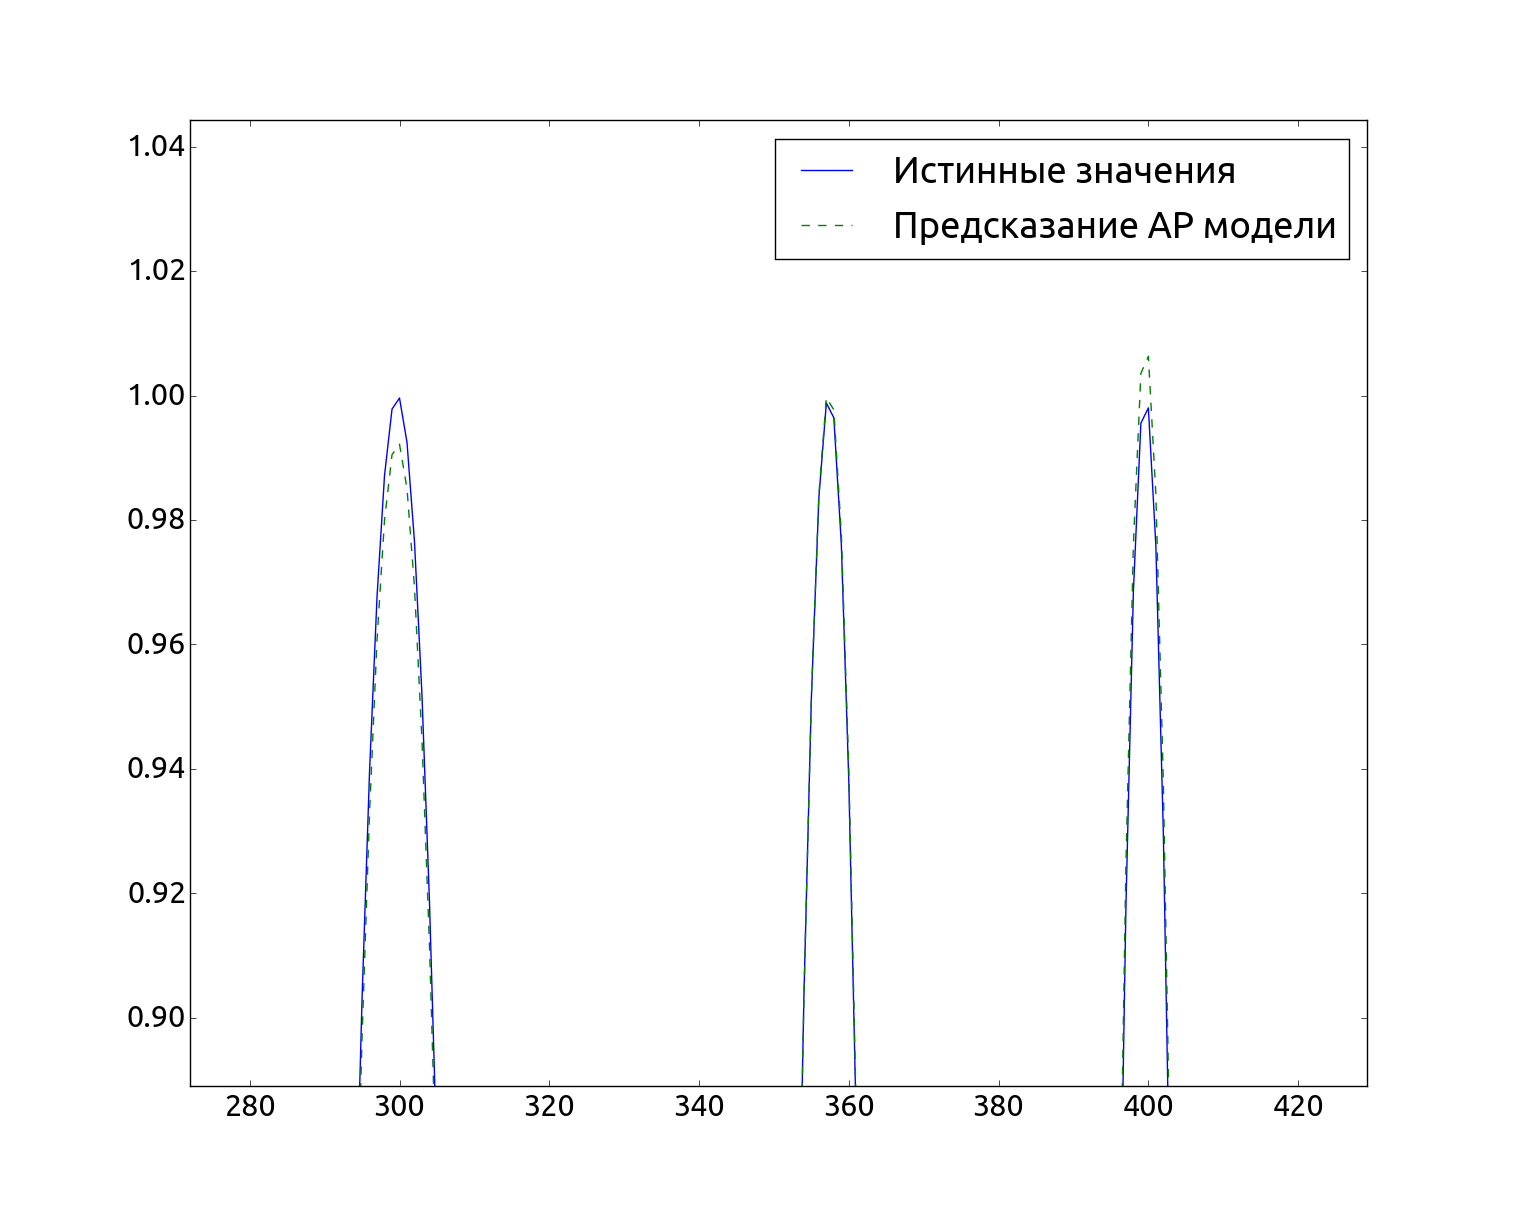
\includegraphics[width=\textwidth]{theory/ar_pred_next_zoomed}
    \caption{}
    \label{fig:theory:ar_pred_next_zoomed}
  \end{subfigure}
  \caption{Предсказания $\AR$ модели на основе реальных данных (\subref{fig:theory:ar_pred_next_whole}). Увеличенный участок графика (\subref{fig:theory:ar_pred_next_zoomed}).}
  \label{fig:theory:ar_pred_next}
\end{figure}

Чтобы построить этот график, были сгенерированы два временных ряда. Оба представляют собой частотно модулированную синусоиду. На первом была настроена $\AR(2)$, а второй использовался для контроля качества. Из него выбирались два последовательных элемента, и модель на их основе предсказывала следующий. Так был составлен ряд предсказаний модели. Как видно, она достаточно хорошо подстроилась под параметры сигнала. Ошибки можно заметить, если увеличить области перегибов синусоиды: сложно угадать точный угол при изменяющейся частоте.

Интересный эффект можно получить, если строить регрессию на ранее предсказанных данных. Ошибка модели накапливается и усиливается со временем, из-за чего сигнал обычно либо угасает, либо устремляется в бесконечность. Поэтому в расчетах стоит использовать только несколько ближайших предсказанных значений. Зато, при появлении новых наблюдений реальных значений не требуется перестраивать модель, ее параметры действительны, если описываемый случайный процесс не изменил своих параметров.

\begin{figure}[h]
  \centering
  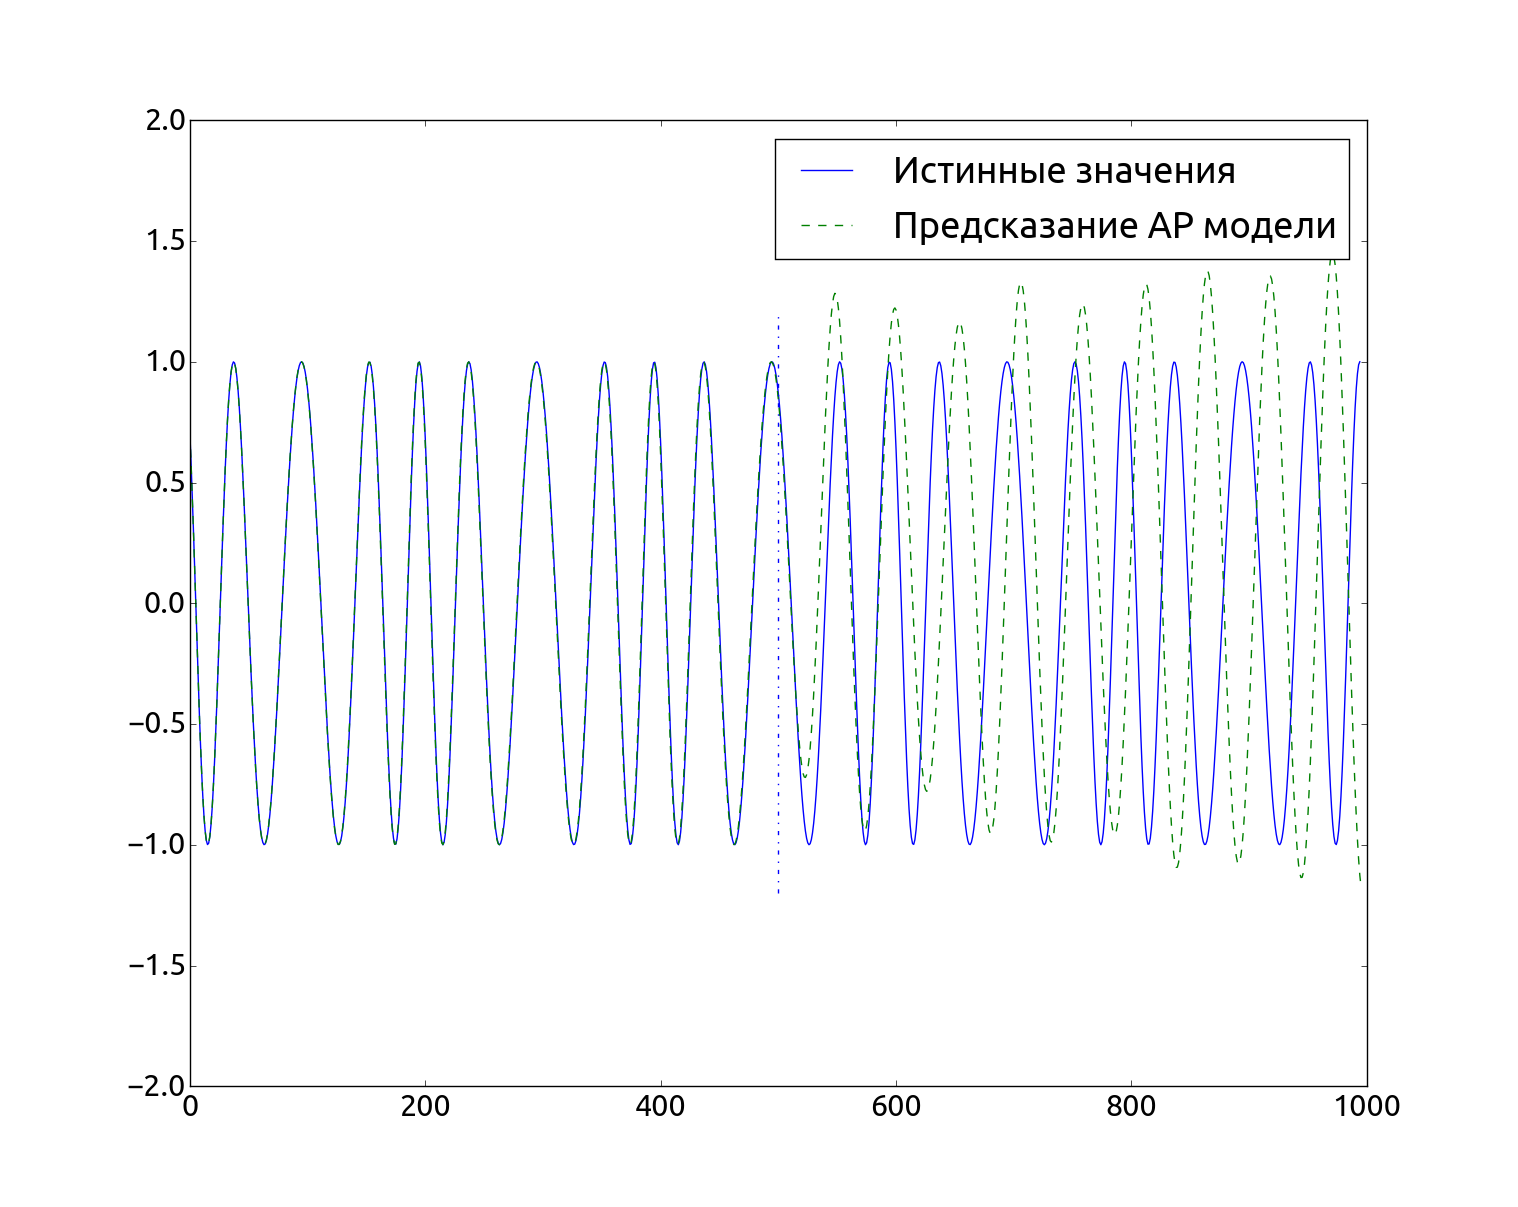
\includegraphics[width=0.9\textwidth]{theory/ar_pred_all}
  \caption{Предсказания $\AR$ модели на основе ранее предсказанных ей значений. Вертикальная линия отмечает начало модельных данных.}
  \label{fig:theory:ar_pred_all}
\end{figure}


\subsection{Модель скользящего среднего}

Авторегрессионная модель непосредственно учитывает абсолютные значения предыдущих наблюдений. Но когда они содержат шум, $\AR$ не может отделить его от сигнала и использует его наравне с полезной информацией. Из-за этого модель становится неустойчивой и качество приближения сильно ухудшается. Для описания шумовых процессов лучше подходит модель скользящего среднего (Moving Average model, $\MA$) (\autoref{eq:theory:ma}). \cite{weber_time_series}

\begin{equation}
  \label{eq:theory:ma}
  X_t = \mu + \varepsilon_t + \sum_{i=1}^q \theta_i \varepsilon_{t-i}
\end{equation}
\begin{explanation}
\item[где] $\mu$ --- константа;
\item $\theta_1, \dotsc, \theta_q$ --- параметры модели;
\item $\varepsilon_t$ --- отклонение в момент времени $t$.
\end{explanation}

Она предполагает, что каждое следующее значение временного ряда выражается линейной комбинацией ошибок предсказаний на предыдущих шагах. Количество параметров называется порядком модели. Модель скользящего среднего $q$-го порядка обозначается $\MA(q)$.

\begin{figure}[h]
  \centering
  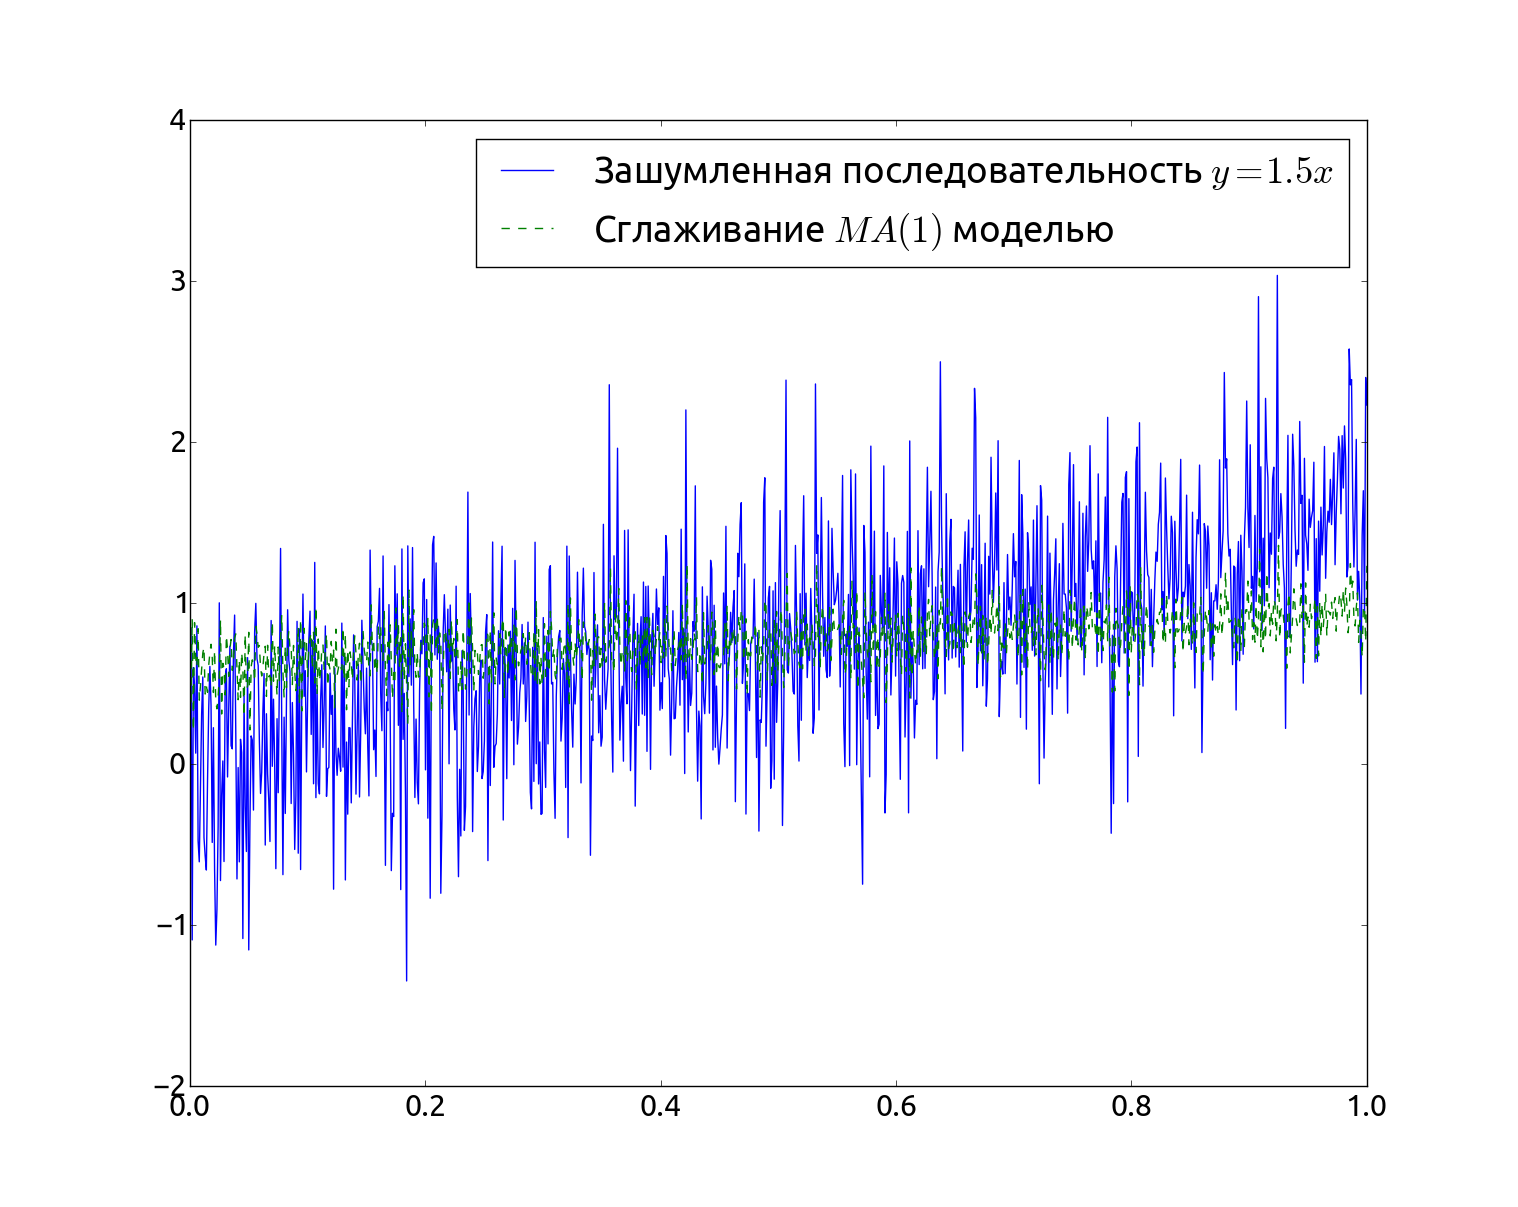
\includegraphics[width=0.9\textwidth]{theory/ma}
  \caption{Применение $\MA$}
  \label{fig:theory:ma}
\end{figure}

После перехода от абсолютных значений к относительным между $\AR$ и $\MA$ осталась некоторая связь. Всякий $\AR(p)$ процесс можно представить как $\MA(\infty)$. Покажем это на примере $\AR(1)$:

\begin{equation}
  \label{eq:theory:ar_as_ma}
  \begin{split}
    X_t & = \phi_1 X_{t-1} + \varepsilon_t \\
        & = \phi_1 (\phi_1 X_{t-2} + \varepsilon_{t-1}) + \varepsilon_t \\
        & = \phi_1 (\phi_1 (\phi_1 X_{t-3} + \varepsilon_{t-2}) + \varepsilon{t-1}) + \varepsilon_t \\
        & \dotso \\
        & = \varepsilon_t + \phi_1 \varepsilon_{t-1} + \phi_1^2 \varepsilon_{t-2} + \phi_1^3 \varepsilon_{t-3} + \dotsb
  \end{split}
\end{equation}

Получилась модель скользящего среднего бесконечно высокого порядка с коэффициентами $\theta_i = \phi_1^i$. Возможен и обратный переход. Это происходит благодаря общему принципу, на которых строятся два подхода --- линейная регрессия над данными из прошлого. Такой подход эффективен, когда нужно определить характеристики случайного процесса, а в наличии есть только его ряд наблюдаемых значений. Принципиально иные методы требуют больше информации, например, несколько коррелированных рядов.

Хотя мы увидели прямую связь между $\AR$ и $\MA$, на практике они обладают разным поведением и применяются для моделирования разных случайных процессов. Так получается, потому что в реальных задачах обычно используются модели невысоких порядков, тогда они имеют разные свойства.

Модель скользящего среднего используется для учета шума во временных рядах. Его невозможно предсказать, но нужно как-то обрабатывать, чтобы он не влиял на работу других моделей. Конечно, полностью избавится от него не удается, но получается уменьшить дисперсию, которую он привносит в процесс.

Как понятно из ее свойств, $\MA$ обычно не применяется сама по себе, а служит для предобработки данных, или как составная часть более сложных систем. Правильная композиция алгоритмов зачастую работает лучше, чем каждая ее составляющая.


\subsection{Модель авторегрессии --- скользящего среднего}

Зная достоинства и недостатки моделей авторегрессии и скользящего среднего, можно заметить, что они взаимодополняют друг друга. Первая неплохо настраивается под параметры случайного процесса, но неустойчива к шуму. Вторая плохо предсказывает сигнал, но сглаживает шумы. Идея их совмещения порождает качественно иную систему, называемую модель авторегрессии --- скользящего среднего ($\ARMA$). \cite{weber_time_series}

\begin{equation}
  \label{eq:theory:arma}
  X_t = c + \varepsilon_t + \sum_{i=1}^p \phi_i X_{t-i} + \sum_{i=1}^q \theta_i \varepsilon_{t-i}
\end{equation}
\begin{explanation}
\item[где] $c$ --- константа;
\item $\varepsilon_t$ --- отклонение в момент времени $t$;
\item $\phi_1, \dotsc, \phi_p$ --- параметры авторегрессии;
\item $\theta_1, \dotsc, \theta_q$ --- параметры скользящего среднего.
\end{explanation}

Формула для $\ARMA$ представляет собой сумму составляющих ее моделей. Получается, каждое значение $X_t$ частично объясняется $\AR$ и частично $\MA$. В идеальном случае первая модель настраивается на полезную информацию, а вторая на шумовые отклонения.

Теперь в уравнении присутствуют и $p$, и $q$, поэтому появляется проблема выбора параметров и их балансировки. Во первых, высокие порядки улучшают качество подгонки под ряд, но ослабляют предсказательную силу модели. Во вторых, не всякая комбинация $p$ и $q$ дает рабочую модель. В процессе настройки параметров многократно решаются задачи оптимизации, а они имеют ограничения относительно своей целевой функции. Часто можно подобрать ряд, на котором эти ограничения не выполняются при заданном порядке модели и обучение модели становится невозможным. Это осложяет применение $\ARMA$ в автоматическом режиме, когда нужно анализировать много совершенно случайных процессов с совершенно различными характеристиками.

\begin{figure}[h]
  \centering
  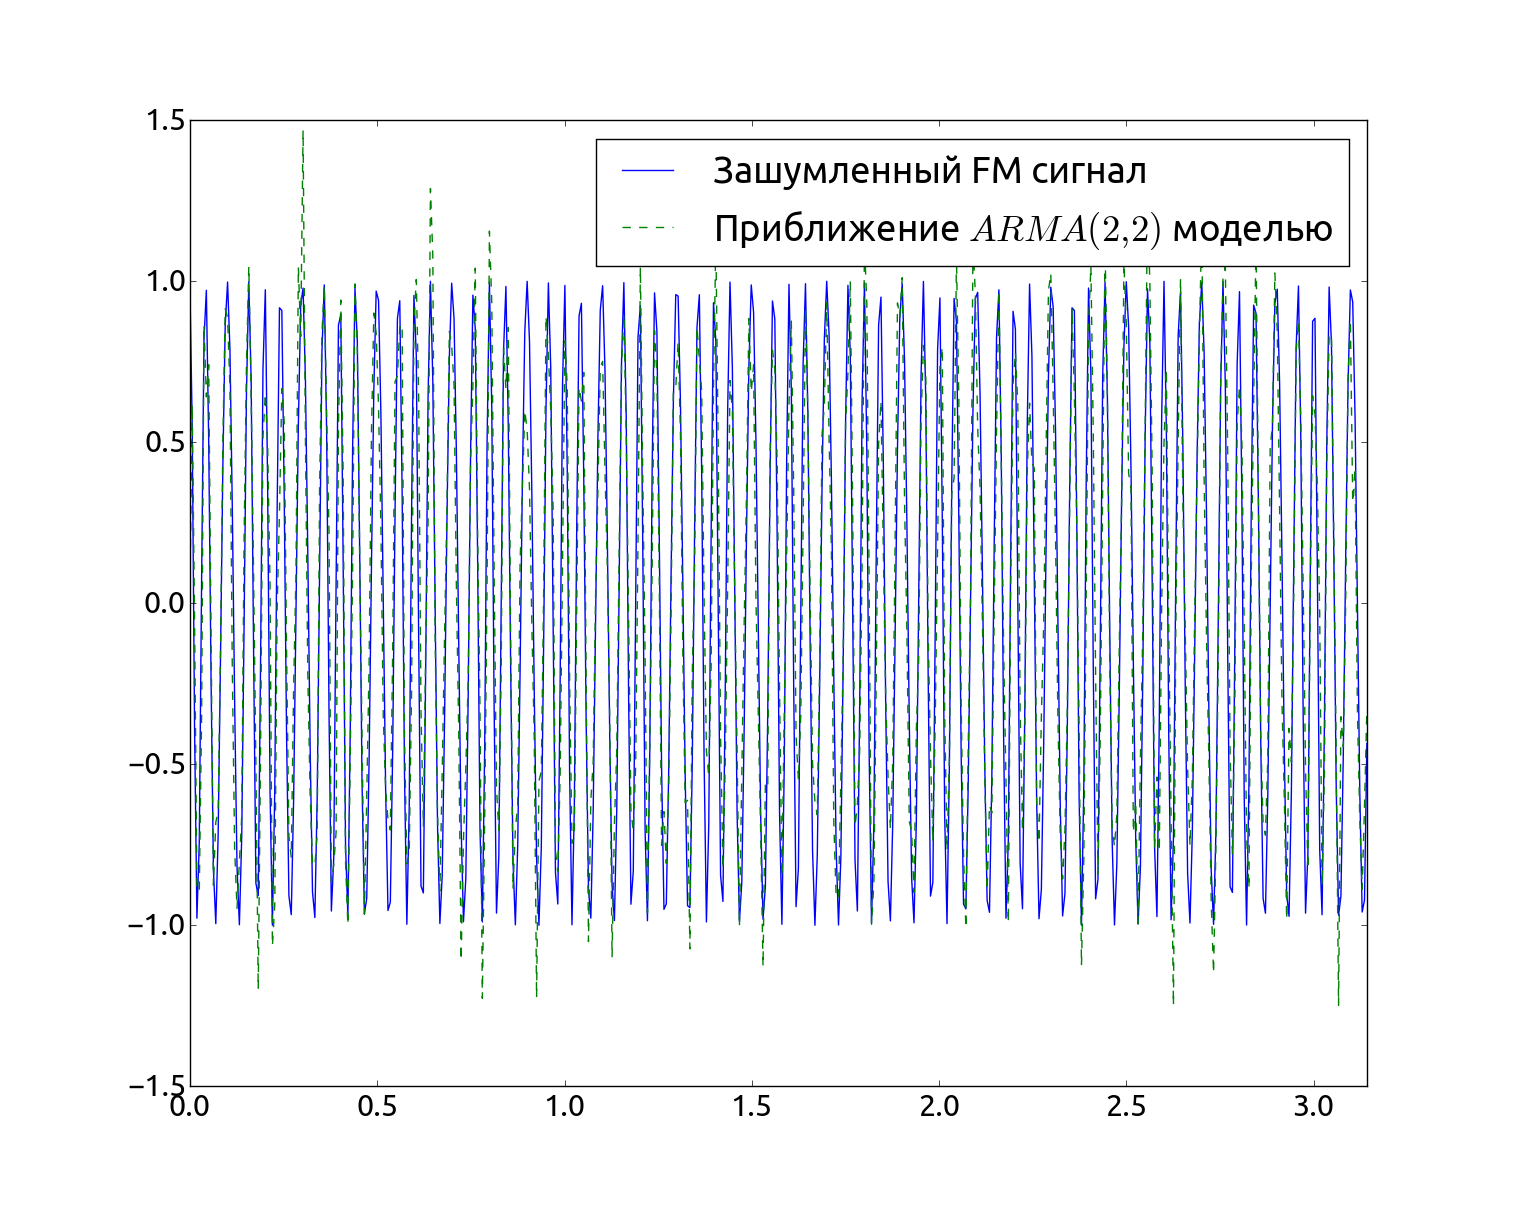
\includegraphics[width=0.9\textwidth]{theory/arma_modelled_fm}
  \caption{Настройка $\ARMA$ под модельный зашумленный FM сигнал}
  \label{fig:theory:arma_modelled_fm}
\end{figure}

На рисунке \ref{fig:theory:arma_modelled_fm} показано, как удается приблизить искусственный FM сигнал, содержащий шум. Видно, что модели не удается угадать точное значение амплитуды и она часто не добирает или выскакивает за реальные значения. Тем не менее, частота приближается достаточно точно, а именно мгновенная частота является определяющей характеристикой FM сигнала. Поэтому, можно сказать, что модель получилась неплохой. Важно заметить, что она настроилась на закономерности, лежащие в основе исходных данных и оказалась слабо подвержена влиянию шума.

\begin{figure}[h]
  \centering
  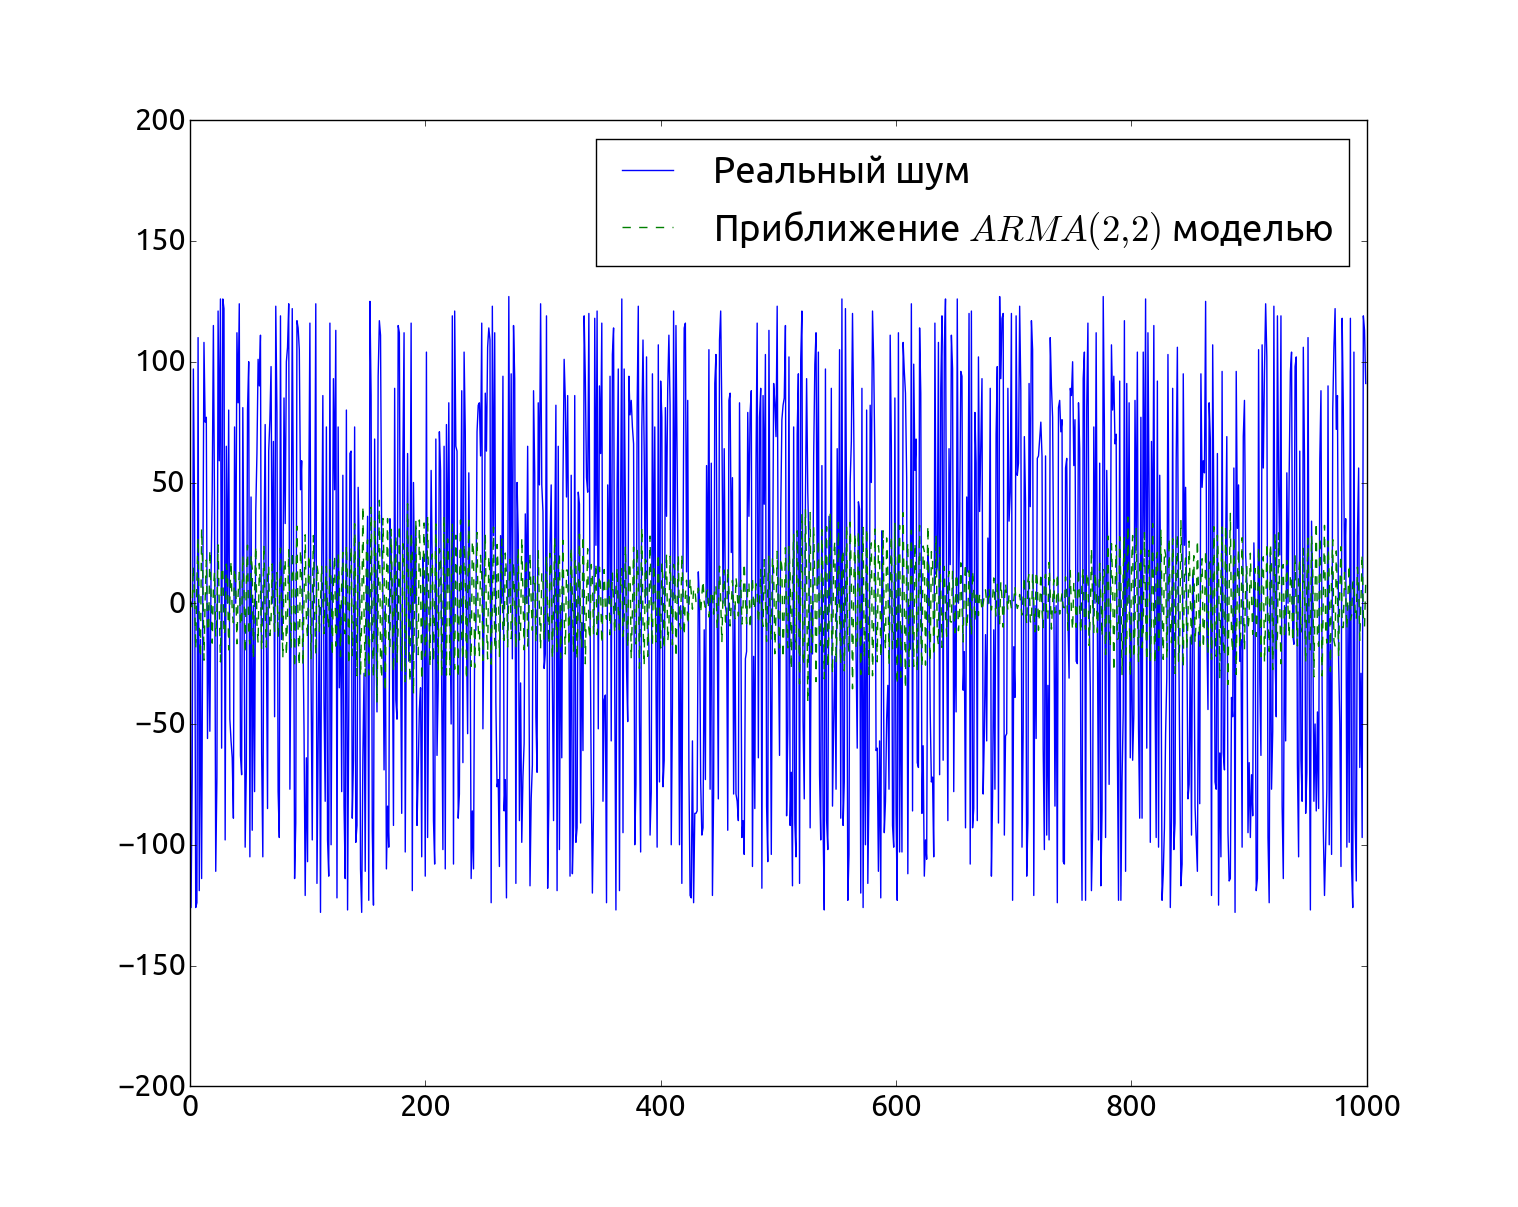
\includegraphics[width=0.9\textwidth]{theory/arma_real_noise}
  \caption{Настройка $\ARMA$ под реальный шум}
  \label{fig:theory:arma_real_noise}
\end{figure}

Для сравнения, на рисунке \ref{fig:theory:arma_real_noise} изображена модель с такими же параметрами, но настроенная на случайный шум. Она уже не приближается к максимальным значениям амплитуды, а колеблется ближе к нулю. Значит, в предсказании больший вес имеет модель скользящего среднего, а для авторегресии не удалось подобрать хороших параметров, поэтому ее влияние было ослаблено. В сравнении этих примеров хорошо видно очень полезное свойство $\ARMA$ --- автоматическое определение параметров приближаемого процесса и гибкая настройка под них. Если в данных есть какой-то сигнал и модель имеет достаточно высокий порядок, то она сумеет подстроиться под него, иначе будет стараться минимизировать ошибку, не отклоняясь далеко от среднего значения.

Этот алгоритм и его модификации нашли широкое применение в эконометрике. Его используют, если временной ряд интерпретируется как случайный процесс, обладающий постоянными на коротком интервале времени параметрами ($\AR$ часть), и испытывающий влияние внешних факторов, не доступных для непосредственного наблюдения ($\MA$ часть). Для этой задачи важна точность предсказания значений ряда в будущем и адаптивность под влияние внешних факторов.

В целях обнаружения сигналов предсказанное значение само по себе не несет полезной информации. Интересно рассмотреть использование $\ARMA$ для различения шумовых и не шумовых сигналов. Можно предположить, что достоверно предсказать информативный сигнал не получится --- для передачи информации нужно часто изменять параметры временного ряда, а модель хорошо работает на слабо стационарных рядах. Следовательно, на не шумовых сигналах ошибка приближения будет велика. Конечно, она будет велика и на случайном шуме, но не всякий шум случаен. Индустриальные помехи могут представлять собой постоянные колебания со слабо меняющейся частотой и мощностью. Эта особенность приближает их к слабо стационарному случайному процессу, который хорошо описывается моделью $\ARMA$. Значит, ее можно применять как фильтр некоторых индустриальных помех, которые по мощности и диапазону частот могут быть похожи на сигнал.

Другое ее применение, о котором уже упоминалось --- обнаружение разладок. Если в полосе частот работают радиосредства, иногда их можно заметить только в период активной передачи информации. В остальное время можно наблюдать только шум, или контрольный сигнал, который бывает сложно отличить от индустриальных помех. В этом случае можно настроить $\ARMA$ на наблюдаемый не информативный ряд. Тогда на предсказанных значения будет более или менее стабильная погрешность. Это говорит о том, что случайный процесс остается неизменным. Если же вдруг наблюдается резкий кратковременный скачок погрешности, это дает повод думать, что по каналу произошла передача информации. Продолжительный анализ повышает достоверность обнаружения. Дополнительным преимуществом метода является низкая вычислительная сложность --- модель достаточно построить один раз, после чего можно осуществлять предсказания по формуле \ref{eq:theory:arma}.

Из-за своей распространенности, методы работы с $\ARMA$ и ее компонентами эффективно реализованы в математических пакетах многих языков программирования. Часто они включают и процедуры выбора оптимального порядка модели. Это позволяет использовать даже в тех алгоритмах, где они играют лишь вспомогательную роль фильтрации или предобработки данных.


\subsection{Спектральный анализ}

Ранее мы рассматривали сигнал как временной ряд, представляющий собой последовательность мгновенных значений его уровня. Это интуитивный подход, который несложен в применении и хорошо изучен в других сферах науки. Проблемы с ним возникают, когда в наблюдаемой полосе частот содержатся несколько сигналов. Каждый из них вносит свой вклад в мгновенные значения уровня, и возникает сложная задача определения компонент сигнала и разделения их. Пример можно увидеть на рисунке \ref{fig:theory:mixed_sins_time}. Там изображен сигнал, состоящий из трех синусоид с разными частотами и амплитудами: $s(t) = 3cos(2\pi 5 t) + 2cos(2\pi 10 t) + 5cos(2\pi 1 t)$. В представлении временного ряда они смешиваются и сложно даже назвать их точное количество, при том что это идеальная модель, не содержащая помех. В реальности проблема оказывается еще серьезнее.

\begin{figure}[h]
  \centering
  \begin{subfigure}{0.45\textwidth}
    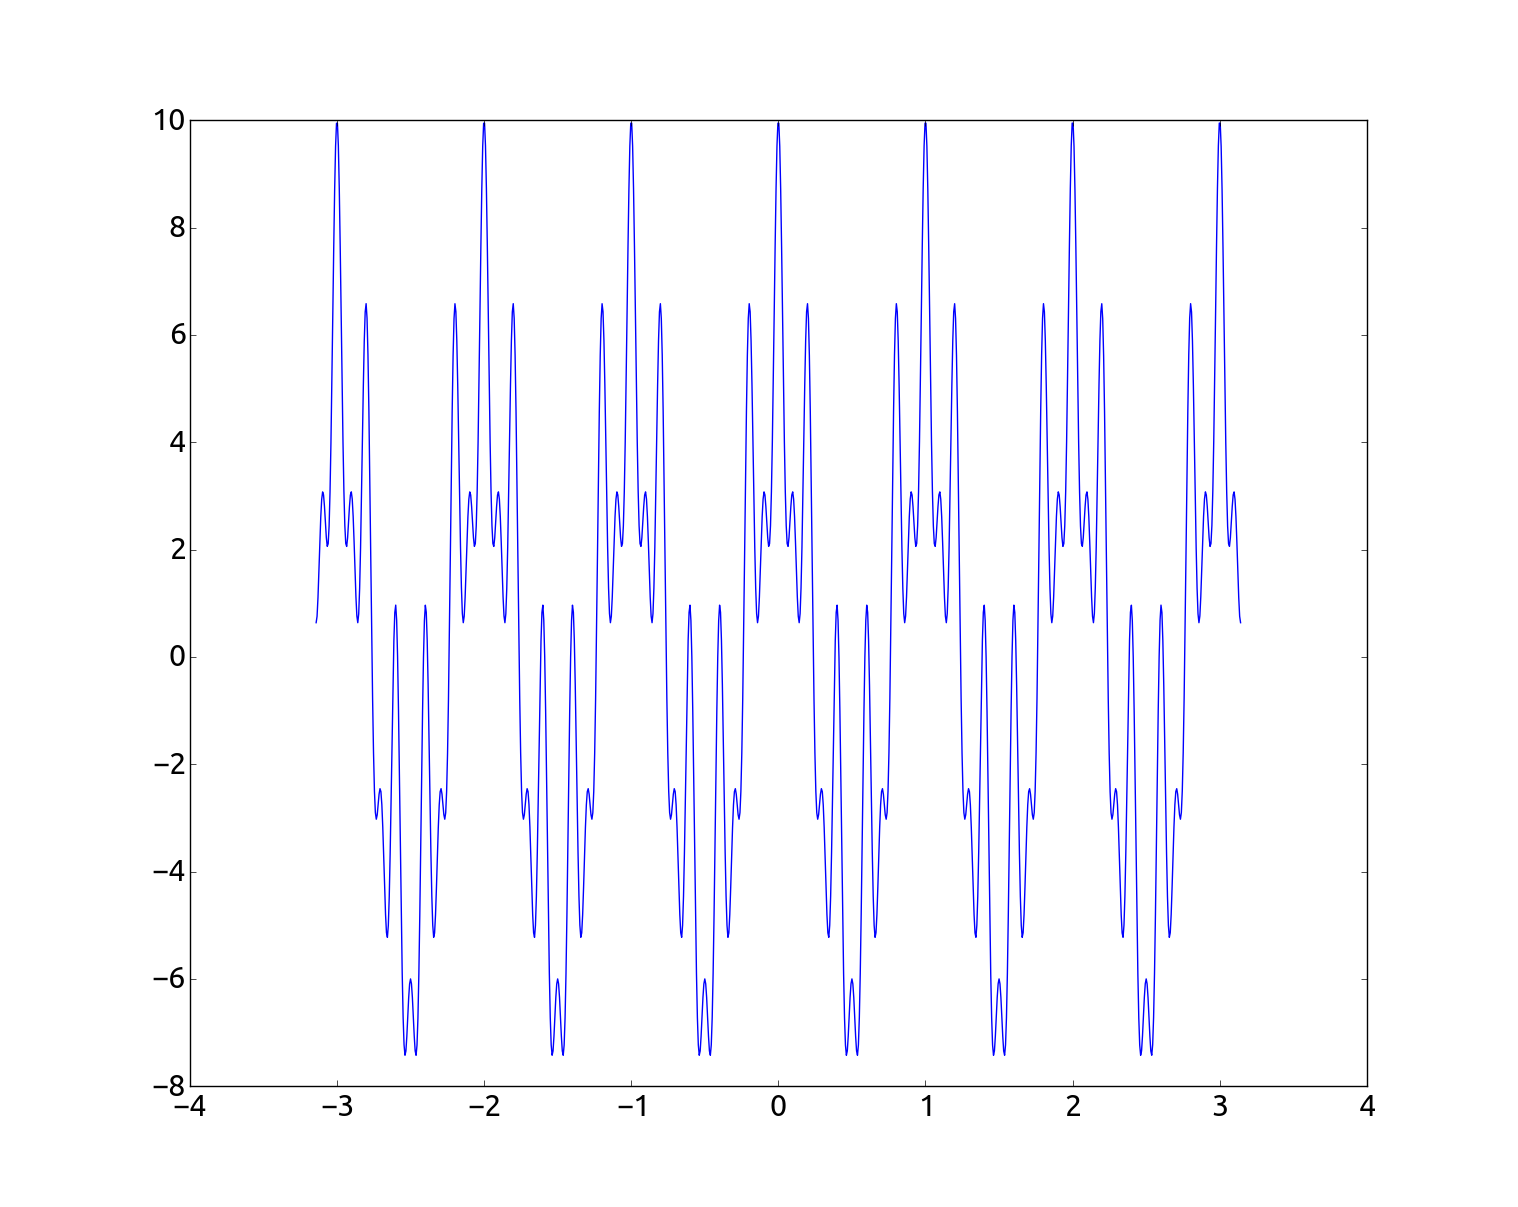
\includegraphics[width=\textwidth]{theory/mixed_sins_time}
    \caption{}
    \label{fig:theory:mixed_sins_time}
  \end{subfigure}
  \begin{subfigure}{0.45\textwidth}
    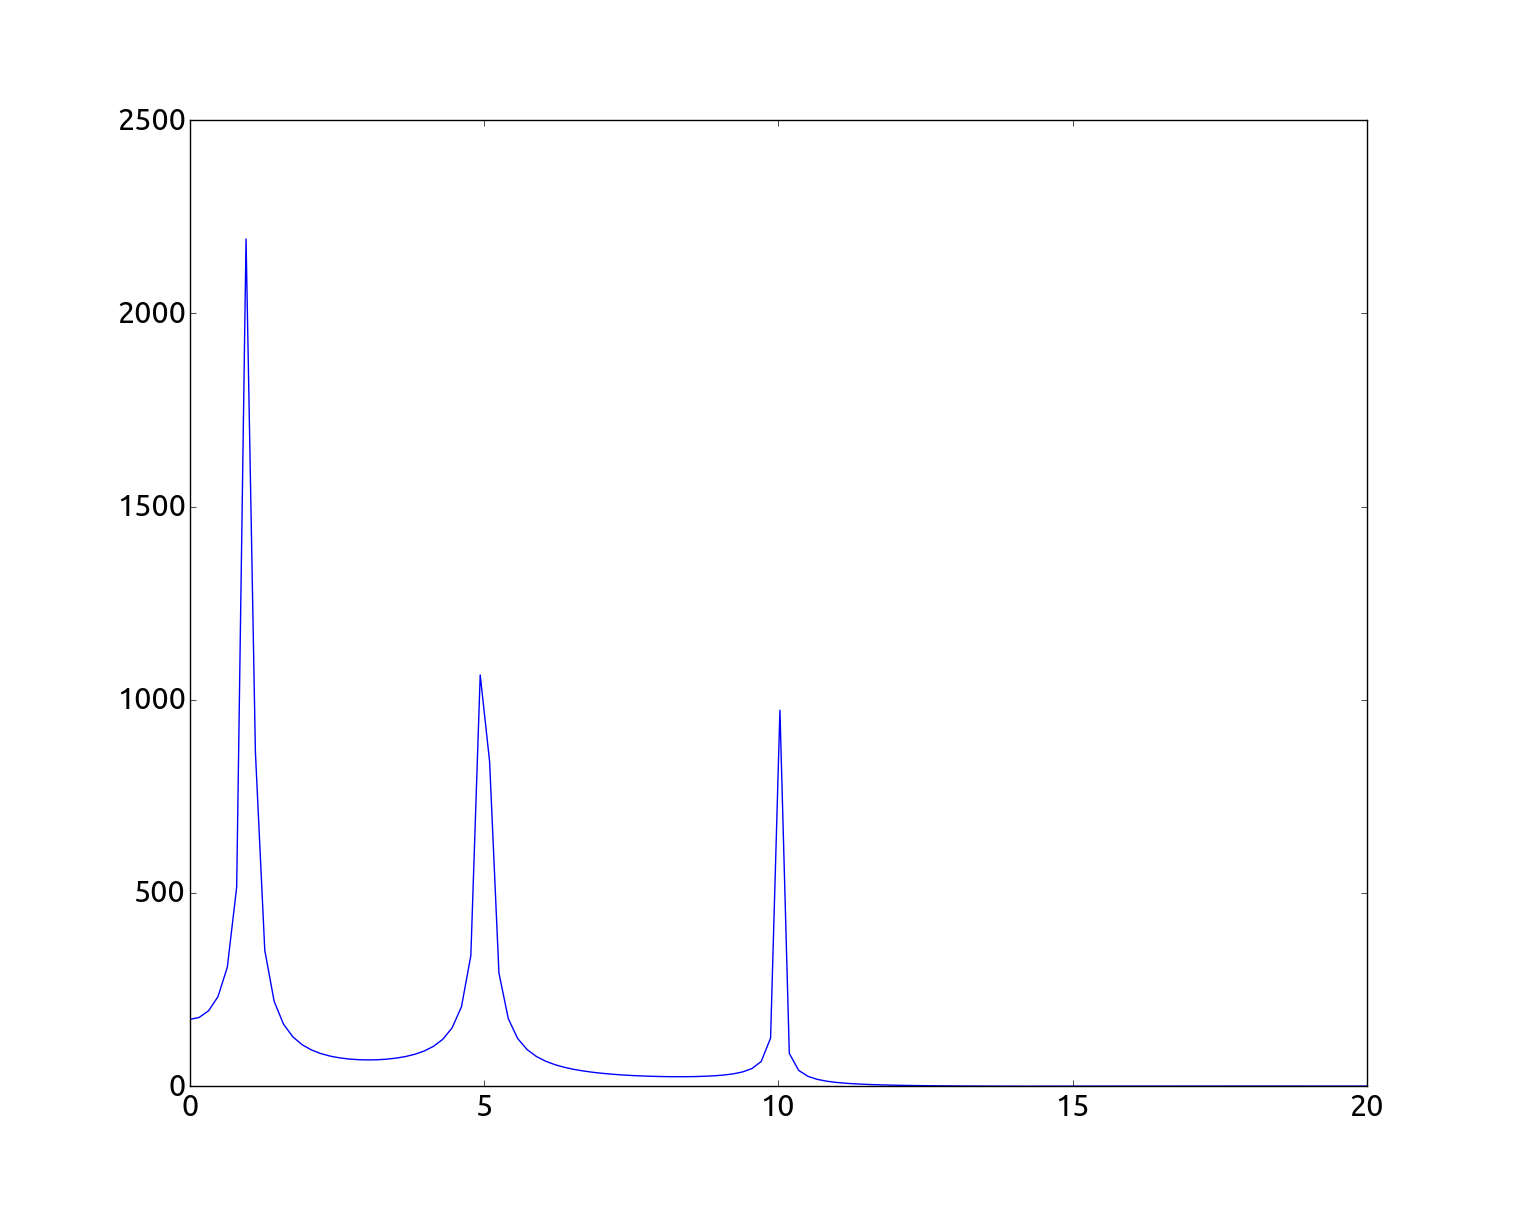
\includegraphics[width=\textwidth]{theory/mixed_sins_freq}
    \caption{}
    \label{fig:theory:mixed_sins_freq}
  \end{subfigure}
  \caption{Смесь синусоид во временном (\subref{fig:theory:mixed_sins_time}) и частотном домене (\subref{fig:theory:mixed_sins_freq})}
  \label{fig:theory:mixed_sins}
\end{figure}

В действительности нам интересно знать, как распределятся энергия сигнала по частотам. Тогда их них можно выделить самые важные и предположить, что в них и заключается вся полезная информация. Этот прием называется переходом из временного домена в частотный и осуществляется с помощью преобразования Фурье. В результате его теряется информация о хронологии значений, но становятся наблюдаемы интегральные энергии гармонических колебаний, присутствующих в сигнале. Частоты, составляющие сигнал называются его спектром, а семейство методов, основывающихся на его изучении --- спектральным анализом.

Если применить преобразование Фурье в предыдущем примере, отдельные синусоиды становятся хорошо разделимы, а их амплитуды сохраняют свои пропорции.

Спектральный анализ очень широко используемая техника. Ее мощь основывается на альтернативном взгляде на наблюдаемое явление. Традиционно мы смотрим на объект в его целостности, приписываем ему неделимые качества. Другой взгляд открывает множество его составных частей, благодаря взаимодействию которых объект имеет те или иные характеристики. Например, исследуя излучение звезд удается определить их химический состав. Это возможно из-за того, что каждый химический элемент имеет характерный для него спектр.

\begin{figure}[h]
  \centering
  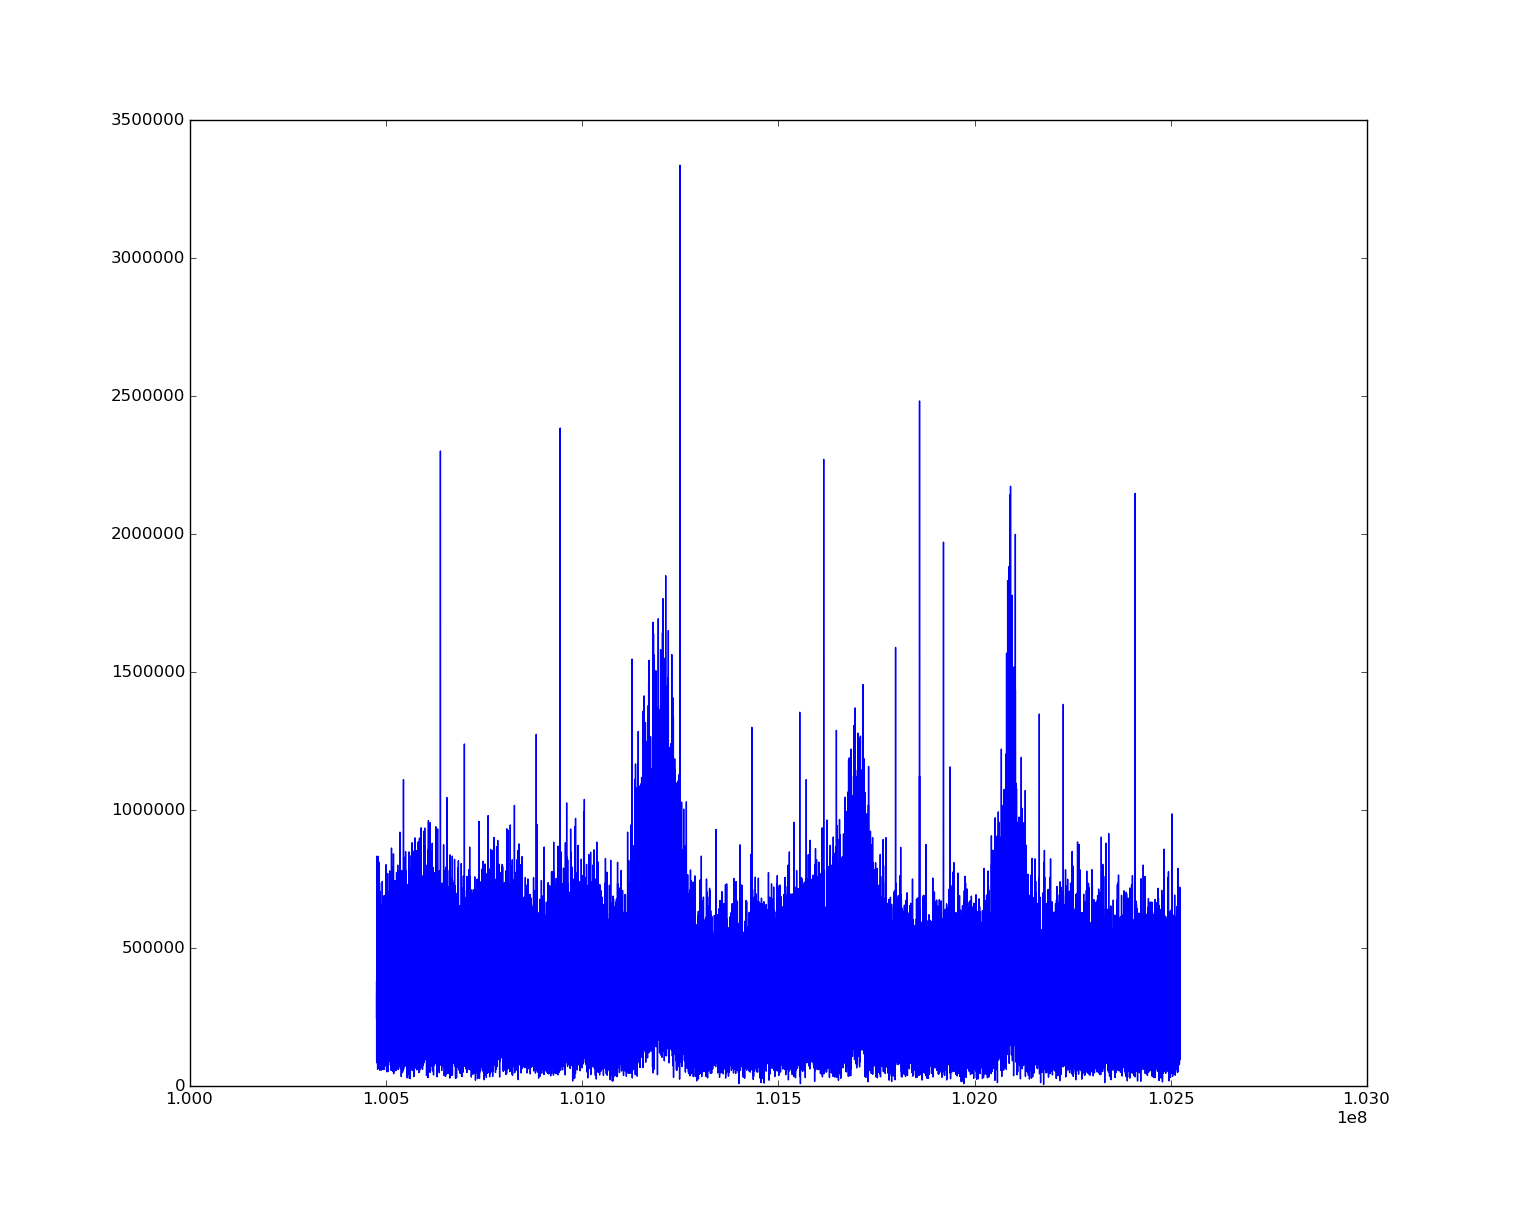
\includegraphics[width=0.9\textwidth]{theory/wfm_freq}
  \caption{Спектр полосы частот, содержащий мощную FM радиостанцию}
  \label{fig:theory:wfm_freq}
\end{figure}

В задачах обнаружения радиосигналов спектральные методы позволяют исследовать широкий диапазон частот. Традиционные радио сканеры "прыгают" по частотам, задерживаясь на каждой лишь несколько долей секунды. За это короткое время они анализируют активность на канале и решают, есть ли там сигнал. Но все остальные частоты в этот момент остаются вне зоны видимости. Из-за такому сканеру может понадобится долгое время для нахождения сигнала рации, которая большую часть времени неактивна. С другой стороны, если используемая аппаратура способна охватить весь интересующий нас диапазон, то применяя спектральный анализ можно исследовать его полностью в каждый момент времени. Это значительно повышает надежность обнаружения.

Работа со спектром широкополосного сигнала лишь общий подход, ставший основой множества конкретных методов. Хотя преобразование и иной взгляд на сигнал сам по себе может подсказать решение несложных проблем (\autoref{fig:theory:wfm_freq}).


\subsection{Преобразование Фурье}

Переход из временного домена в частотный осуществляется с помощью преобразования Фурье ($\FT$). Это интегральное преобразование одной функции комплексной переменной в другую, которая описывает коэффициенты при разложении исходной на элементарные составляющие --- гармонические колебания с разными частотами (\autoref{eq:theory:fourier}). \cite{dspguide} \cite{fourier_habr} \cite{fourier_wiki}

\begin{equation}
  \label{eq:theory:fourier}
  \FT(f) = \hat{f}(\xi) = \int\limits_{-\infty}^{\infty} f(x) e^{-2 \pi i x \xi} \mathrm{d}x
\end{equation}

Понять суть преобразования достаточно просто, если вспомнить, что $e^{-2 \pi i x \xi}$ --- это комплексная форма записи "виртуального" гармонического колебания частоты $\xi$. Реальный синус и косинус выражаются как комбинация таких колебаний. Тогда для фиксированного $\xi$ берется сумма поточечных произведений сигнала и абстрактной гармоники в каждый момент времени. Если они согласованы по частоте, то произведение в большинстве случаев будет положительно, а их пики будут примерно совпадать и давать большие значения при умножении. Иначе произведение будет положительным и отрицательным в примерно равной пропорции, а их сумма будет колебаться вблизи нуля. Поэтому, если в сигнале присутствует гармоника частоты $\xi$, ей будет соответствовать большое значение $\hat{f}(\xi)$. Отношение этих значений друг к другу можно интерпретировать как относительный вклад, который гармоника делает в общую мощность сигнала.

Преобразование Фурье обратимо (\autoref{eq:theory:inv_fourier}). Это позволяет применять ряд методов, которые переводят функцию в частотный домен, осуществляют над ее спектром некоторые преобразования и возвращаются обратно к временному ряду. Так, например, можно программно реализовать фильтры высоких и низких частот.

\begin{equation}
  \label{eq:theory:inv_fourier}
  f(x) = \int\limits_{-\infty}^{\infty} \hat{f(\xi)} e^{2 \pi i \xi x} \mathrm{d}\xi
\end{equation}

На практике обычно имеется конечная последовательность наблюдений уровня сигнала, а не его аналитическая функция. В этом случае применяется адаптированный алгоритм --- дискретное преобразование Фурье (ДПФ) (\autoref{eq:theory:discrete_fourier}). В дальнейшем, говоря о преобразовании Фурье, мы будем иметь в виду именно его.

\begin{equation}
  \label{eq:theory:discrete_fourier}
  X_k = \sum_{n=0}^{N-1} x_n e^{\frac{-2 \pi i}{N} k n} \quad k = 0, \dotsc, N-1
\end{equation}

Спектр, полученный с помощью ДПФ имеет одну неизбежную особенность: если шаг дискретизации равен $\Delta x$, то спектр будет периодической функцией с периодом $T = \frac{1}{\Delta x}$, где спектр выборки заключен в одном периоде, а вне его только повторяется. Для реального сигнала, он к тому же будет симметричен относительно нуля, поэтому обычно изображают только положительную половину одного периода.

\begin{figure}[h]
  \centering
  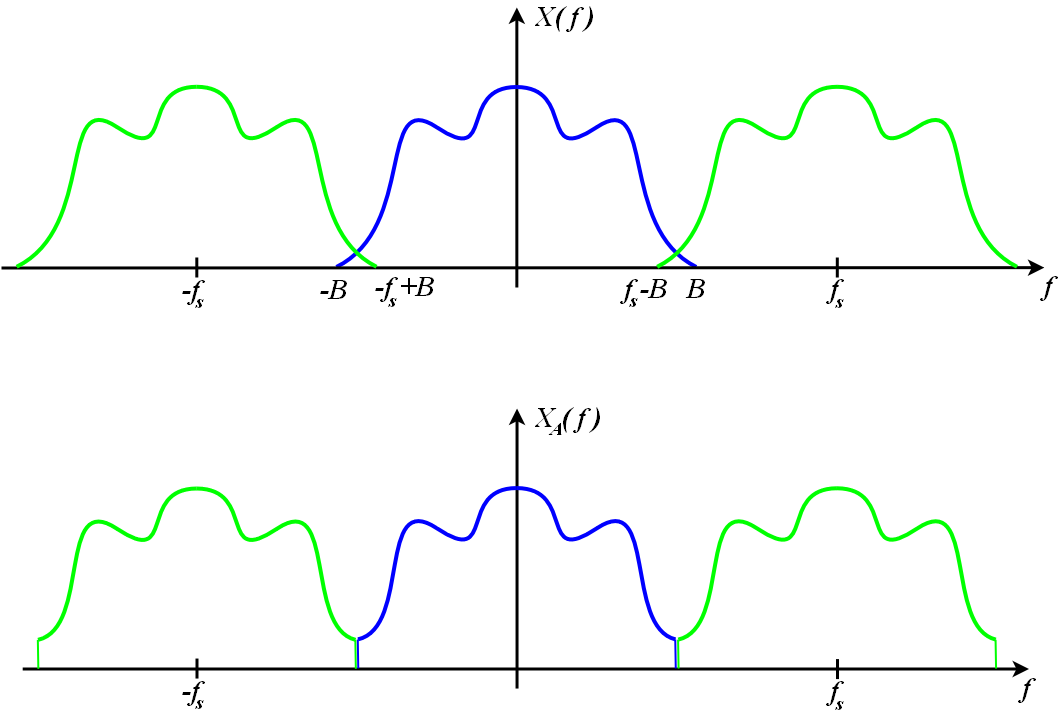
\includegraphics[width=0.9\textwidth]{theory/aliasing}
  \caption{Алиасинг}
  \label{fig:theory:aliasing}
\end{figure}

Эта особенность может привести к нежелательным искажениям спектра при неправильном семплировании. Теорема Котельникова утверждает, что частота дискретизации должна быть не менее чем в два раза выше максимальной частоты, содержащейся в сигнале. Если это требование не выполняется, его спектр становится шире $\frac{1}{\Delta x}$, происходит алиасинг. Периоды спектра смешиваются и становится невозможным восстановить его исходную форму (\autoref{fig:theory:aliasing}). Причем он соответствует спектру другой правильно семплированной последовательности. Чтобы избежать этого, нужно убедиться, что сигнал не содержит слишком высоких частот. Для этого перед семплированием нужно применять ВЧ фильтр.


\subsection{Частотно-временное представление}

Исследование спектра сигнала является мощным инструментом его анализа. Но и у него есть свои недостатки. Преобразование Фурье --- это интегральное преобразование, то есть оно комбинирует все значения функции в одно. В случае радиосигнала это значит, что все мгновенные значение мощность будут свернуты в одно --- спектральную мощность гармоники частоты $\xi$. При этом теряется история изменения сигнала. Это не большая проблема, если составляющие его частоты имеют примерно одинаковую мощность на протяжении всего времени наблюдения. Но реальные сигналы обычно не обладают таким свойством. Они могут изменяться во времени, прекращаться и появляться вновь. Его хронологию невозможно увидеть в спектре. \cite{cohen_tfa}

Для иллюстрации возьмем два различных сигнала. Оба составлены из одинаковых гармоник, расположенных в разном порядке (\autoref{eq:theory:combined1}) и (\autoref{eq:theory:combined2}).

\begin{equation}
  s_1(t) =
  \begin{cases}
    cos(2 \pi 5 t) & \quad 0 \leq t < \frac{\pi}{3} \\
    cos(2 \pi 17 t) & \quad \frac{\pi}{3} \leq t < \frac{2\pi}{3} \\
    cos(2 \pi 31 t) & \quad \frac{2\pi}{3} \leq t < \pi
  \end{cases}
  \label{eq:theory:combined1}
\end{equation}

\begin{equation}
  s_2(t) =
  \begin{cases}
    cos(2 \pi 31 t) & \quad 0 \leq t < \frac{\pi}{3} \\
    cos(2 \pi 17 t) & \quad \frac{\pi}{3} \leq t < \frac{2\pi}{3} \\
    cos(2 \pi 5 t) & \quad \frac{2\pi}{3} \leq t < \pi
  \end{cases}
  \label{eq:theory:combined2}
\end{equation}

Очевидно их различие. Оно также наблюдается во временном представлении (\autoref{fig:theory:combined1_time} и \autoref{fig:theory:combined2_time}). Но спектр этих двух сигналов практически идентичен (\autoref{fig:theory:combined1_freq} и \autoref{fig:theory:combined2_freq}). Эта особенность ограничивает множество выводов, которые можно делать основываясь только на частотном представлении.

\begin{figure}[h]
  \centering
  \begin{subfigure}{0.45\textwidth}
    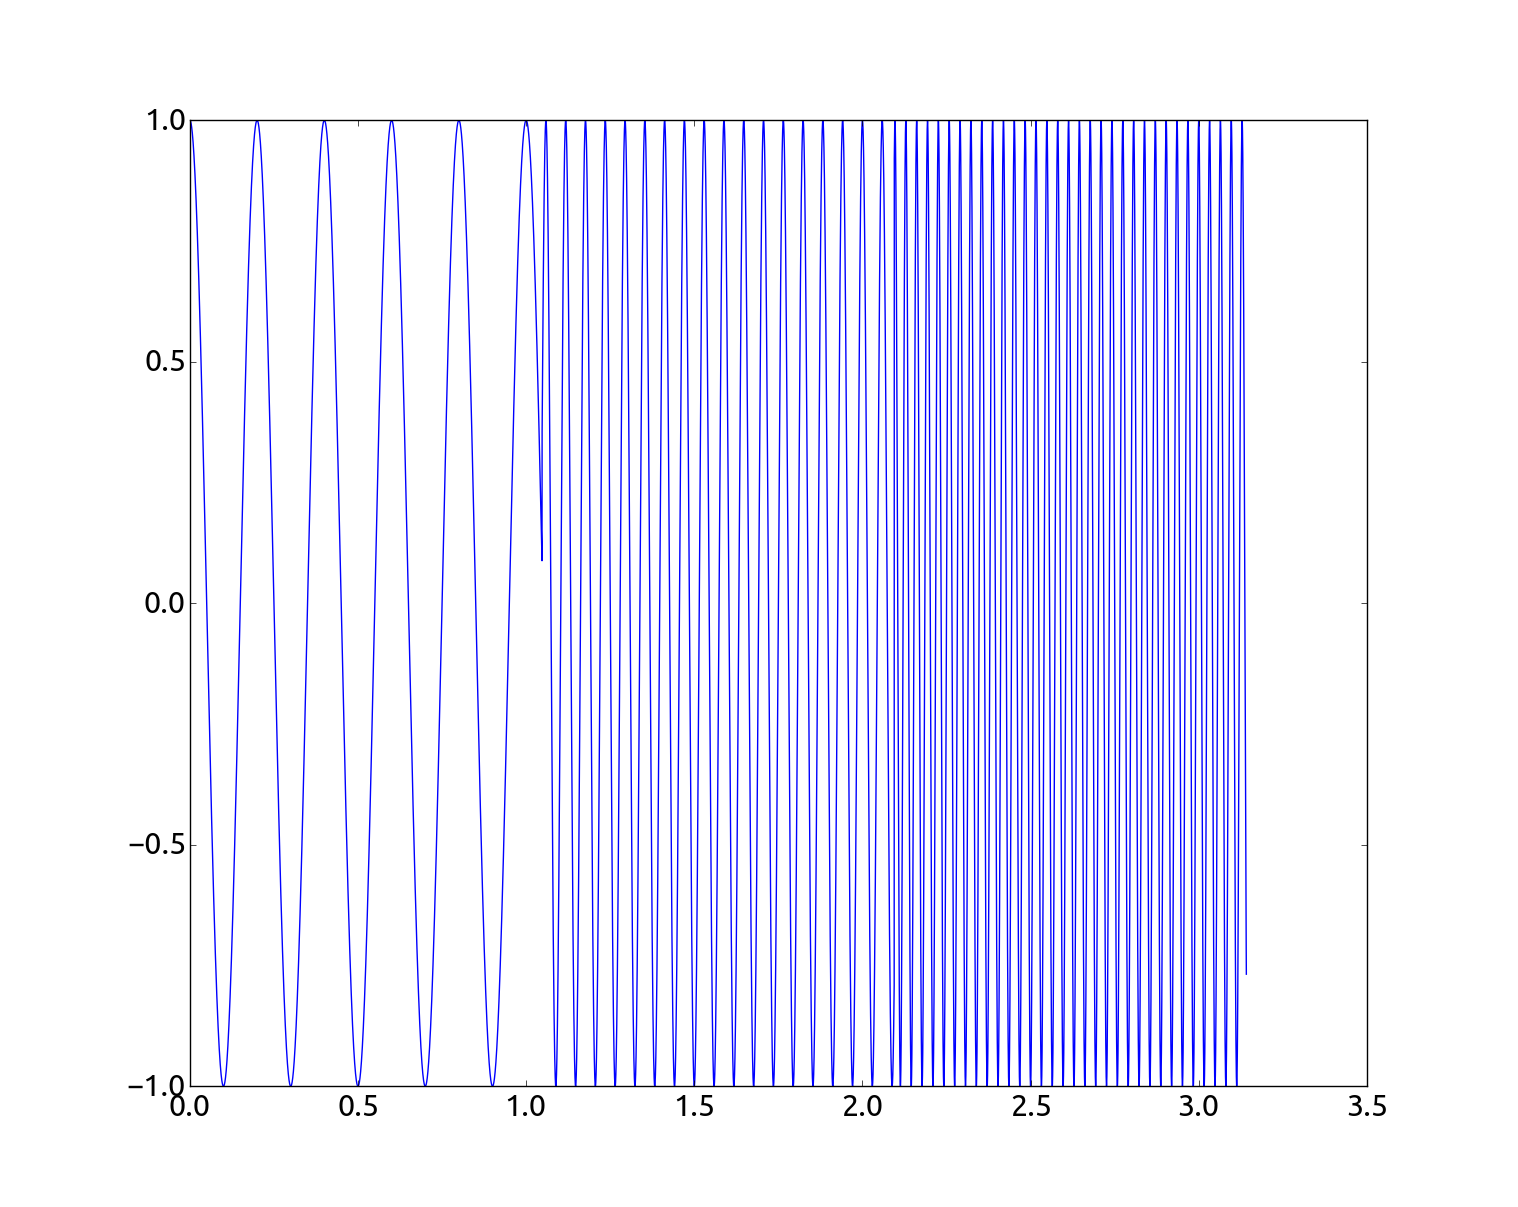
\includegraphics[width=\textwidth]{theory/combined1_time}
    \caption{}
    \label{fig:theory:combined1_time}
  \end{subfigure}
  \begin{subfigure}{0.45\textwidth}
    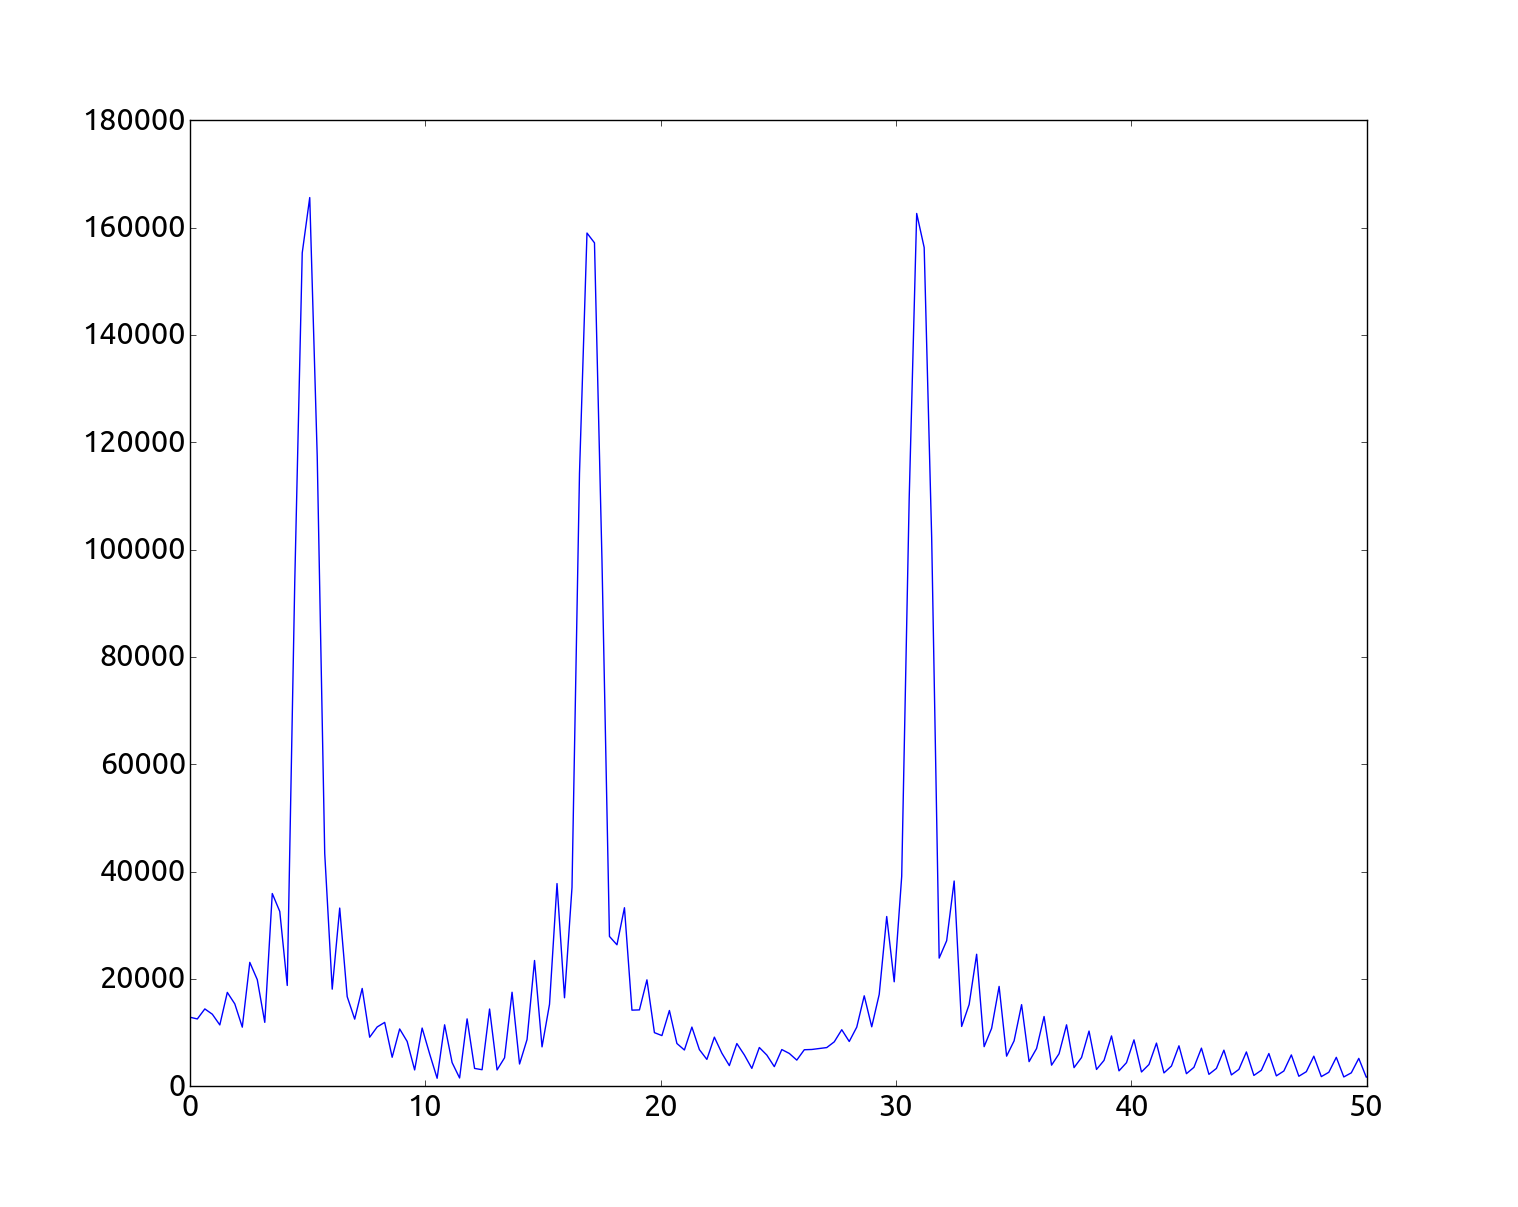
\includegraphics[width=\textwidth]{theory/combined1_freq}
    \caption{}
    \label{fig:theory:combined1_freq}
  \end{subfigure}
  \caption{Временное (\subref{fig:theory:combined1_time}) и частотное (\subref{fig:theory:combined1_freq}) представление $s_1$}
  \label{fig:theory:combined1}
\end{figure}

\begin{figure}[h]
  \centering
  \begin{subfigure}{0.45\textwidth}
    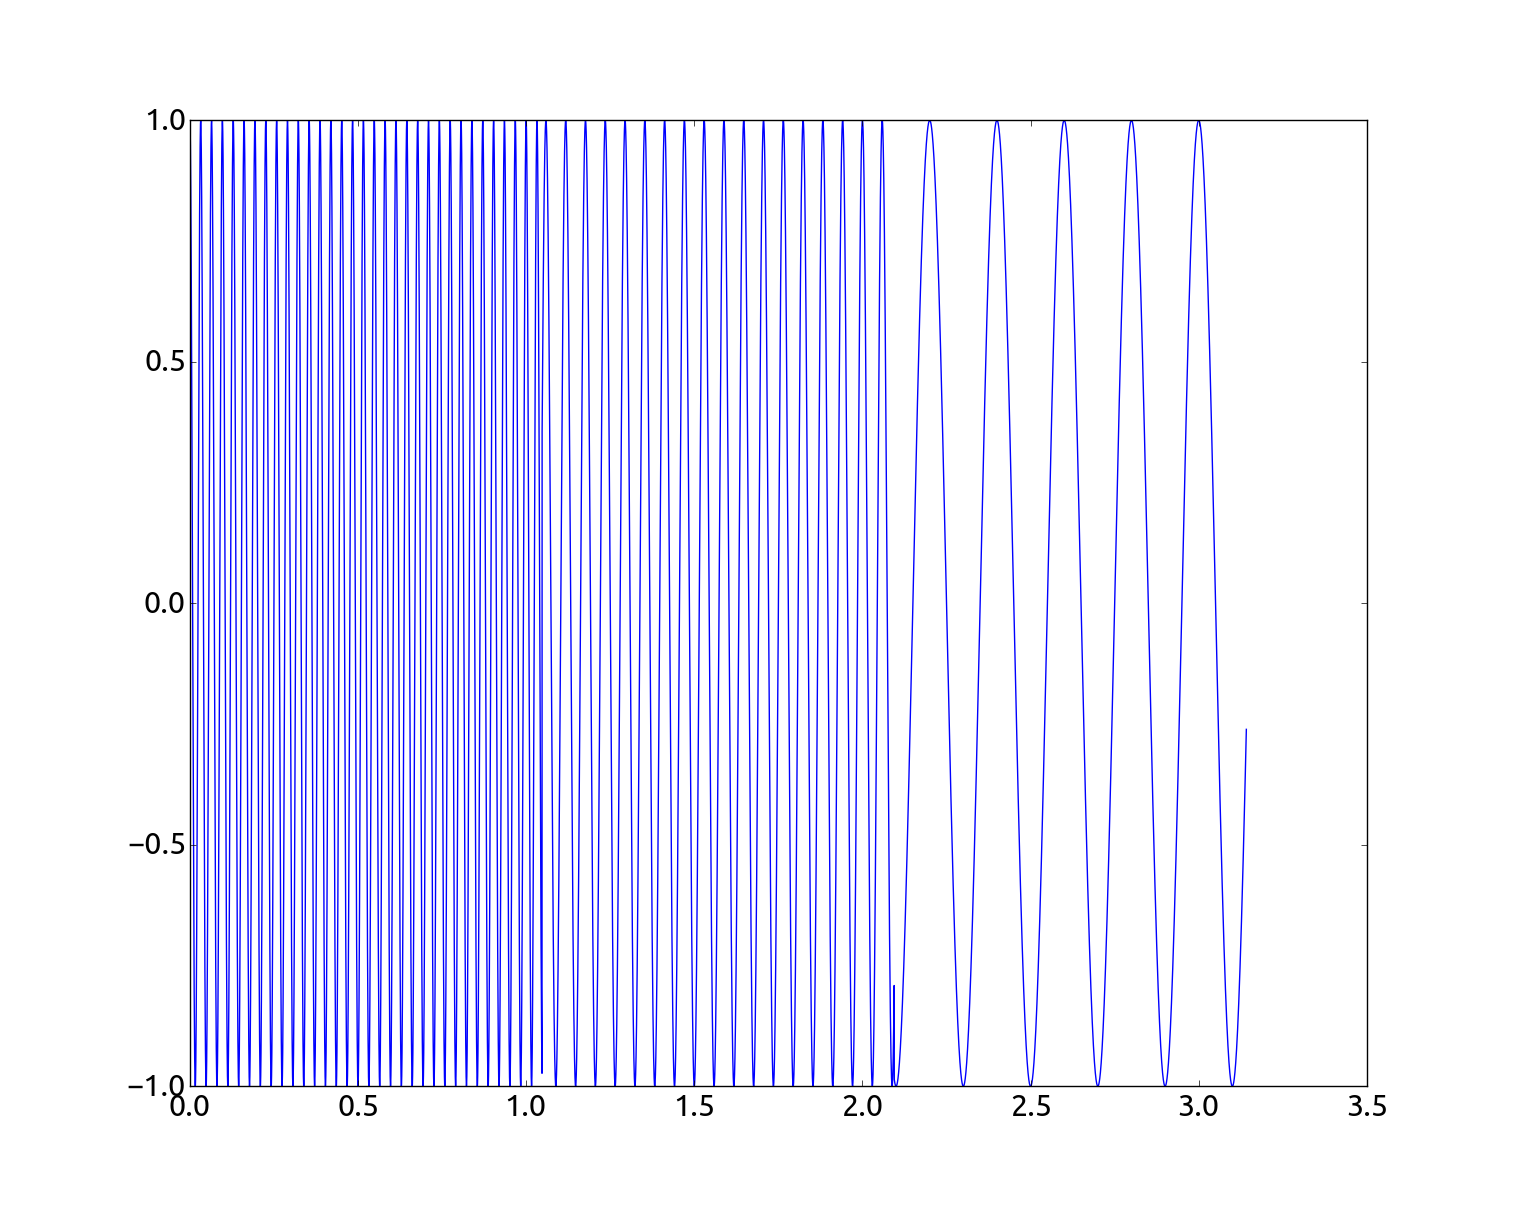
\includegraphics[width=\textwidth]{theory/combined2_time}
    \caption{}
    \label{fig:theory:combined2_time}
  \end{subfigure}
  \begin{subfigure}{0.45\textwidth}
    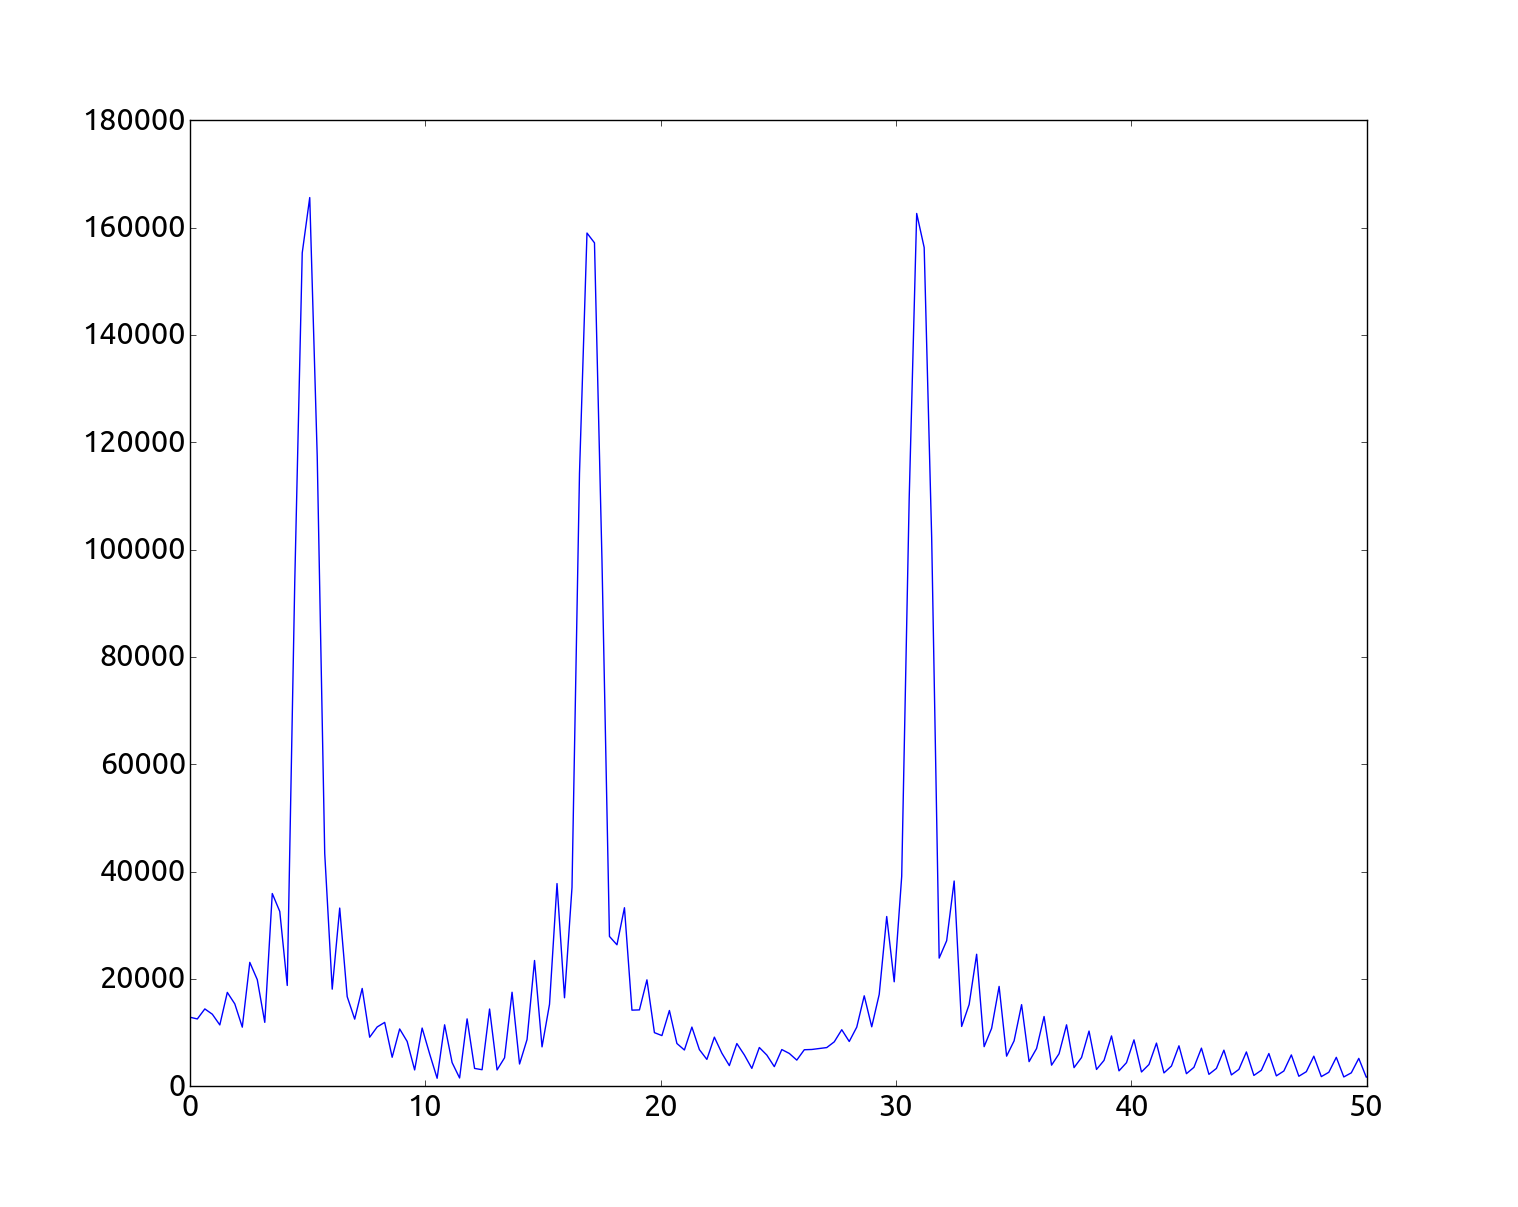
\includegraphics[width=\textwidth]{theory/combined2_freq}
    \caption{}
    \label{fig:theory:combined2_freq}
  \end{subfigure}
  \caption{Временное (\subref{fig:theory:combined2_time}) и частотное (\subref{fig:theory:combined2_freq}) представление $s_2$}
  \label{fig:theory:combined2}
\end{figure}

Другая проблема --- это периодически возникающие сигналы, когда активность в полосе частот наблюдается только во время обмена информацией. Преобразование Фурье будет усреднять ее с периодами бездействия, усложняя задачу обнаружения. В таком режиме работают многие рации и другие устройства служебной связи, что делает спектральный анализ неоптимальным методом.

Решение предлагают частотно-временные преобразования. Они отвечают на вопрос, какова была мощность гармоники с частотой $\xi$ в момент времени $t$. Визуально его можно отобразить в осях частота-время, где яркость каждой точки соответствует спектральной мощности.

Применительно к предыдущему примеру такой подход дает возможность увидеть последовательность синусоид во времени (\autoref{fig:theory:combined_stfts}). Он совмещает лучшее из временного и частотного представления, но и имеет недостатки, о которых будет сказано позже.

\begin{figure}[h]
  \centering
  \begin{subfigure}{0.45\textwidth}
    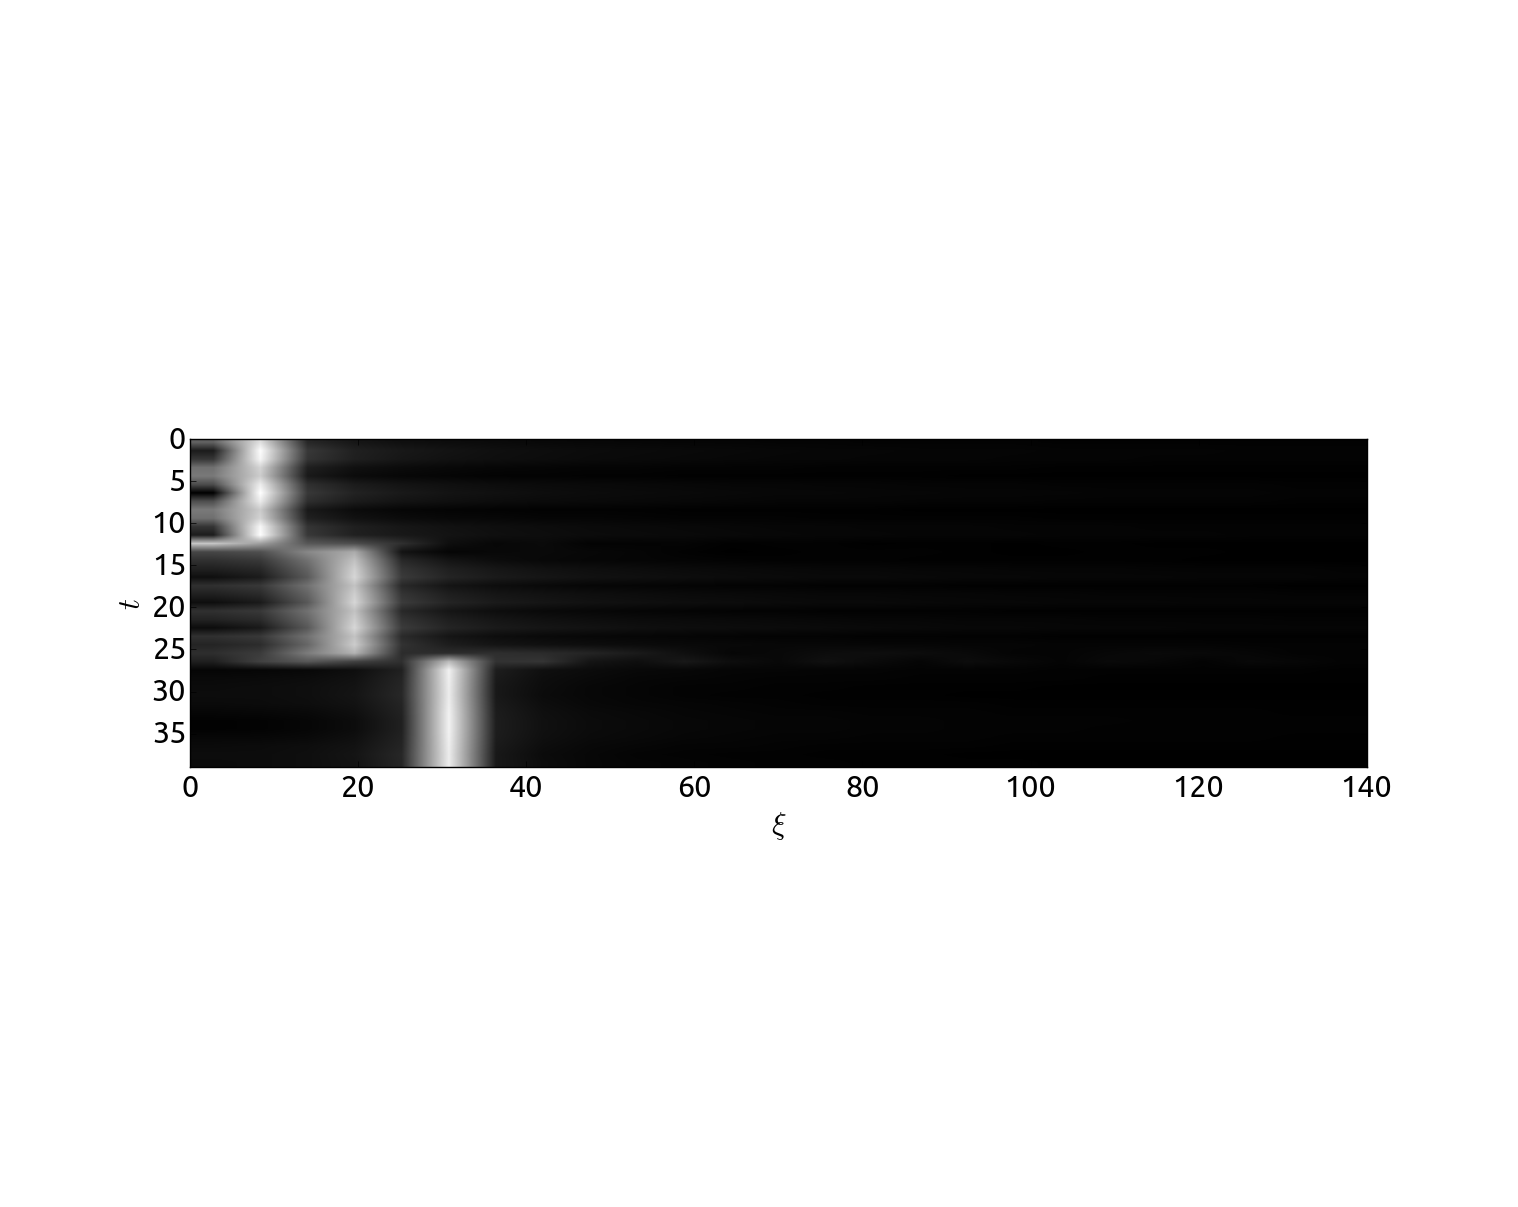
\includegraphics[width=\textwidth]{theory/combined1_stft}
    \caption{}
    \label{fig:theory:combined1_stft}
  \end{subfigure}
  \begin{subfigure}{0.45\textwidth}
    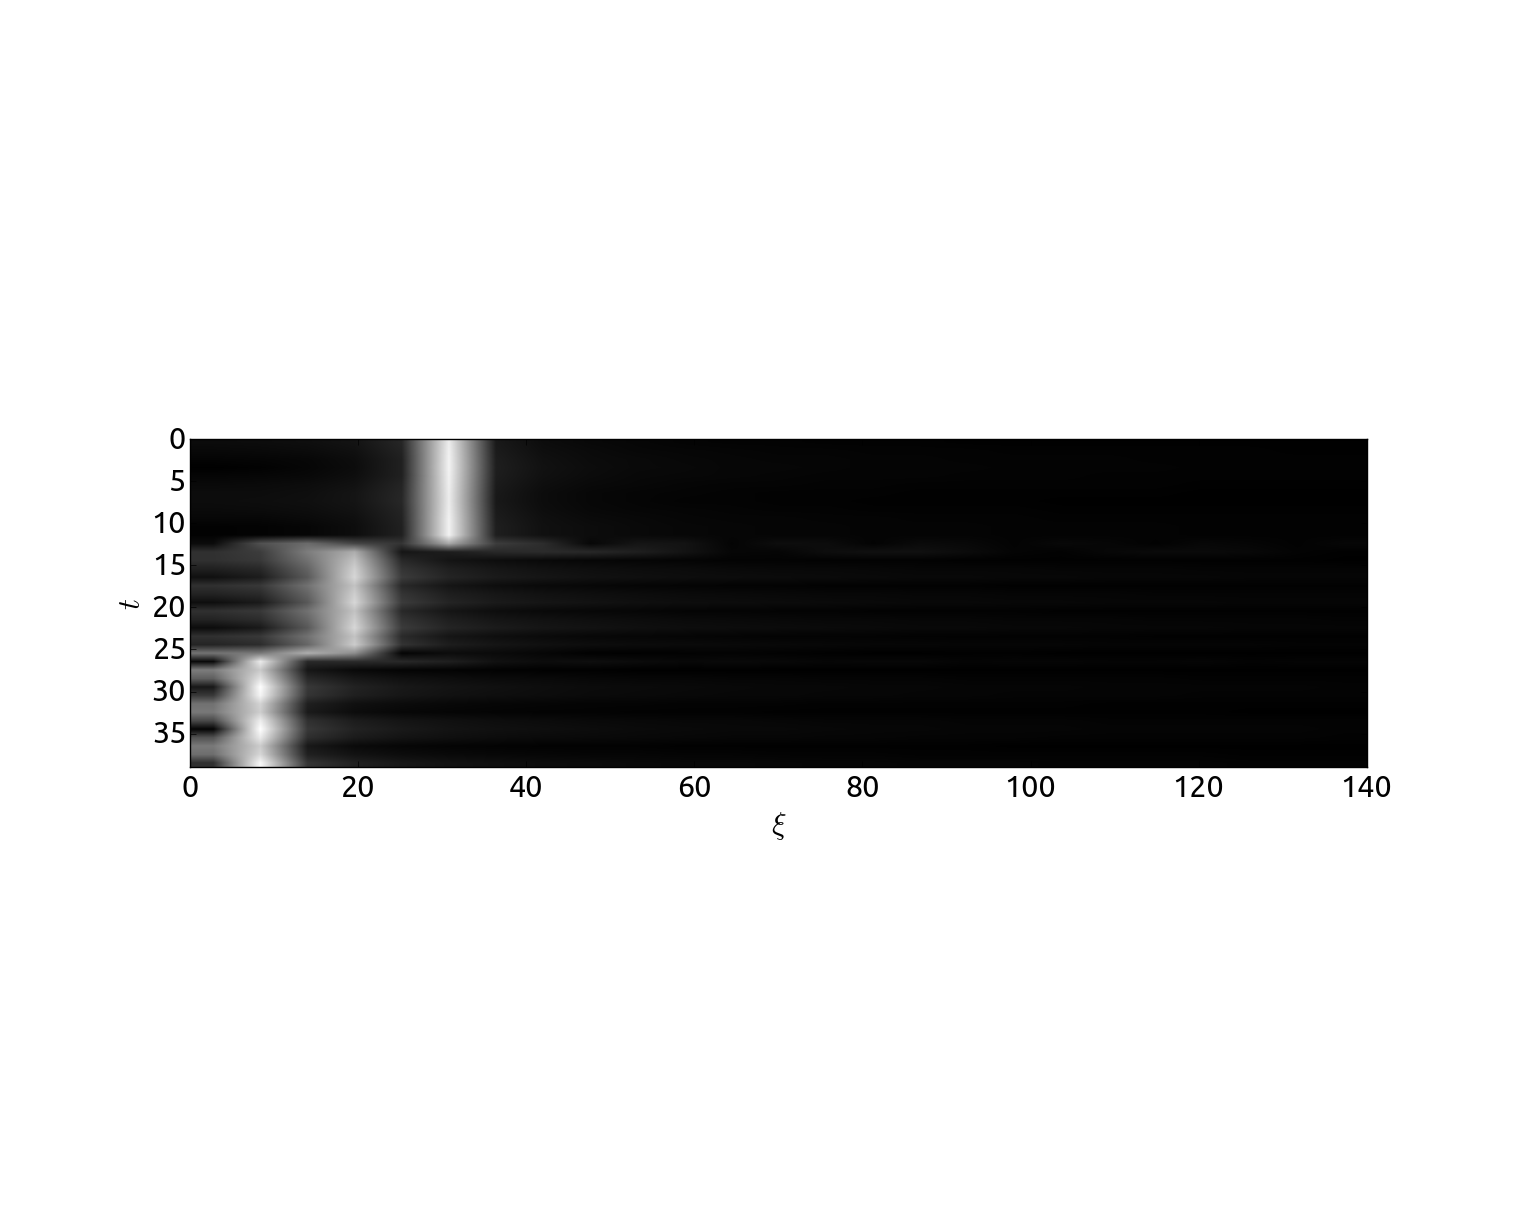
\includegraphics[width=\textwidth]{theory/combined2_stft}
    \caption{}
    \label{fig:theory:combined2_stft}
  \end{subfigure}
  \caption{Частотно-временное представление $s_1$ (\subref{fig:theory:combined1_stft}) и $s_2$ (\subref{fig:theory:combined2_stft})}
  \label{fig:theory:combined_stfts}
\end{figure}


\subsection{Оконное преобразование Фурье}

Базовым инструментом для представления спектра во времени является оконное преобразование Фурье. Его идея заключается в том, что вместо одного ДПФ, оперирующего на всей последовательности, можно произвести несколько на ее участках. По получившемуся множеству спектров узнается, с определенной точностью, частотный состав сигнала в разные промежутки времени. Более того, каждое преобразование выполняется над окном, примененным к последовательности. Настраивая параметры окна можно изменять характеристики локальных спектров (\autoref{eq:theory:stft}). \cite{stft_wiki}

\begin{equation}
  \label{eq:theory:stft}
  \mathit{STFT}(x(t))(m, \xi) = X(m, \xi) = \sum_{n=-\infty}^\infty x(n) w(n - m) e^{-j \xi n}
\end{equation}
\begin{explanation}
\item[где] $w(n - m)$ --- оконная функция с центром в $m$.
\end{explanation}

Этот метод прост и был открыт достаточно давно, но широко используется до сих пор из-за интерпретируемости и вычислительной эффективности.

Теперь, когда мы работаем с частями последовательности, возникает проблема потери точности. Согласно свойствам преобразования Фурье, поточечное умножение функции на окно равносильно свертке их спектров. Это значит, что применяя любое окно, мы производим свертку спектра и вводим в него новые побочные значения. Это явление получило название спектральной утечки. Ее симптом --- появление нежелательных пиков, окружающих настоящий (боковых лепестков). С отдалением от центра они затухают, но вблизи могут быть сравнимы с оригиналом.

Чтобы ослабить эффект спектральной утечки нужно подобрать подходящие параметры окна. В первую очередь это его ширина. Слишком узкое окно помимо утечки вызовет размытие спектра. Когда последовательность, к которой применяется преобразование Фурье слишком коротка, ее можно описать большим числом различных гармоник, из-за чего частоты становятся хуже различимы. Увеличение длины последовательности уменьшает "<двусмысленность"> и обеспечивает четкое различение частот. С другой стороны, при слишком широком окне теряется смысл частотно-временного представления, так как снижается его разрешающая способность --- слишком длительные промежутки времени оказываются объединены. Природа преобразования требует компромисса между детализацией по времени и частоте. Это делает затруднительным его применение к сигналам, динамичным в обоих осях.

Второй по значимости фактор --- это форма окна. Существует множество оконных функций, обладающих разными свойствами. Самым простым является прямоугольное, которое не меняет форму функции в своих пределах, а вне их обнуляет ее. Его особенность в резком "обрыве" на краях, что может ухудшить качество преобразования, в частности, их-за высоких боковых лепестков. Популярны разновидности окна Хэмминга, имеющего куполообразную форму. Оно не имеет недостатков прямоугольного окна, но уменьшает эффективную длину выборки, что требует установки большей ширины.

Участки на границах окна всегда отображаются недостаточно четко, поэтому нужно предусматривать перекрытие и не доверять значениям в приграничной области. Перекрытие можно делать сколь угодно большим, оно будет только "растягивать" временную ось, повышая детализацию спектра.


\subsection{Сверточные нейронные сети}

Задачу обнаружения сигналов можно свести к задаче бинарной классификации. Действительно, если рассматривать каждый тип сигнала по отдельности, то для заданной спектрограммы можно спросить, присутствует он в ней или нет. Тогда для $N$ разновидностей сигналов можно построить $N$ классификаторов, отвечающих на этот вопрос.

Нейронные сети применяются для этих целей с середины прошлого века. Однако, признание пришло к ним лишь в последние годы с появлением сверточных НС, которые осуществили прорыв в области распознавания изображений, превысив на некоторых наборах данных средний результат человека.

Спектрограмму также можно рассматривать как растровое изображение, где вертикальная ось --- это время, горизонтальная --- частота, а значение пикселя --- моментальная мощность сигнала на частоте. Тогда к ней можно применить распознавание нейронной сетью. Преимущества такого подхода в том, что сеть способна автоматически подстроиться под особенности каждого типа сигнала и в случае изображений делает это значительно лучше чем написанные человеком алгоритмы.

\begin{figure}[h]
  \centering
  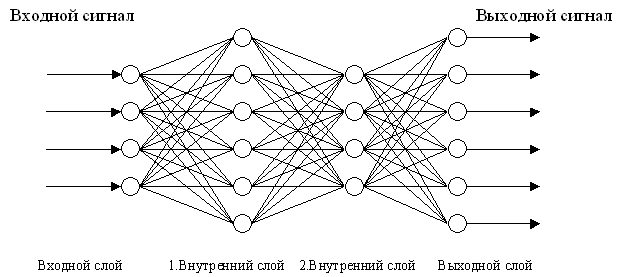
\includegraphics[width=0.9\textwidth]{theory/nn}
  \caption{Нейронная сеть с двумя скрытыми слоями}
  \label{fig:theory:nn}
\end{figure}

Структура обычной сети изображена на рисунке \ref{fig:theory:nn}. Она имеет входной слой, который соответствует необработанным данным, скрытые слои, вычисляющие некоторую функцию от входных данных и выходной слой, представляющий результаты работы. Каждый нейрон применяет заданную функцию к данным, поступающим на вход и отдает ее результат на выход. В простейшем случае он подсчитывает взвешенную сумму аргументов. Обучением сети называется подбор оптимальных параметров (весов), с которыми достигается минимальная ошибка. После обучения сеть можно применять к новым данным.

\begin{figure}[h]
  \centering
  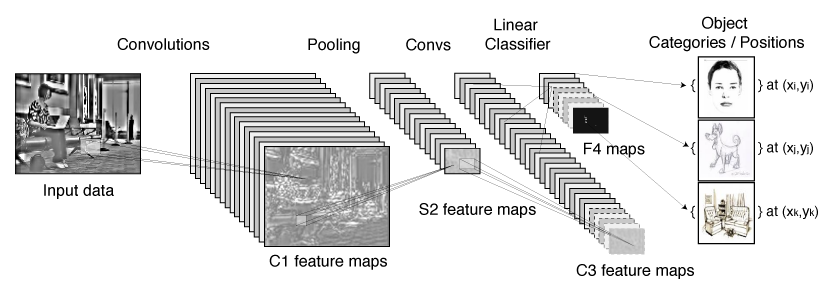
\includegraphics[width=0.9\textwidth]{theory/cnn}
  \caption{Принцип работы сверточной нейронной сети}
  \label{fig:theory:cnn}
\end{figure}

Нейронные сети столь долгое время оставались в неизвестности из-за того, что из традиционная структура плохо подходит для работы с двухмерными данными. Сначала их надо линеаризовать, в результате чего теряется истинная мера близости между точками. Этот критический недостаток удалось преодолеть лишь в начале двухтысячных годов с изобретением сверточных НС (\autoref{fig:theory:cnn}). Их особенность заключается в применении операции свертки в нейронах первых слоев. Она выполняется над двумерным окном изображения, которое учитывает пространственную близость отдельных пикселей, и способна на основании этого находить и использовать новые закономерности в данных. \cite{cnn_wiki}

Появление сетей такого типа вызвало резкий рост качества в задачах классификации изображений. Оно приблизилось к возможностям человека.
Стоит отметить, что идея этой конструкции была позаимствована из нейробиологии. Она соответствует представлениям ученых о принципах работы зрительных клеток.

На первых слоях сверточная нейронная сеть выделяет некоторые примитивные формы --- углы, градиенты цвета, и т.д. На последующих они используются для построения более сложных фигур. Оказывается, изображение определенного объекта состоит из присущей именно ему комбинации таких фигур. Сложная структура сети способна разложить картинку на составляющие и по ним определить исходный объект.

Можно предположить, что такой подход окажется эффективным и в случае спектрограмм различных сигналов. Каждая их них обладает своими уникальными особенностями, которые способна обнаружить и использовать сеть.

К сожалению, это метод не был испытан в дипломном проекте из-за нехватки времени. Но успех сверточных нейронных сетей в близких областях дает основания ожидать от них высокой достоверности обнаружения.
